%
% The first command in your LaTeX source must be the \documentclass command.
\documentclass[sigchi]{acmart}

%
% defining the \BibTeX command - from Oren Patashnik's original BibTeX documentation.
\def\BibTeX{{\rm B\kern-.05em{\sc i\kern-.025em b}\kern-.08emT\kern-.1667em\lower.7ex\hbox{E}\kern-.125emX}}
    
% Rights management information. 
% This information is sent to you when you complete the rights form.
% These commands have SAMPLE values in them; it is your responsibility as an author to replace
% the commands and values with those provided to you when you complete the rights form.
%
% These commands are for a PROCEEDINGS abstract or paper.
\copyrightyear{2022}
\acmYear{2022}
\setcopyright{acmlicensed}
\acmConference[SNA '22]{Social Network Analysis '22}{2021/22}{University of Pisa, Italy}
\acmBooktitle{Social Network Analysis '22}
\acmPrice{0.00}
%\acmDOI{10.1145/1122445.1122456}
%\acmISBN{978-1-4503-9999-9/18/06}

\usepackage{adjustbox}
\usepackage{caption}
\usepackage{subcaption}

% end of the preamble, start of the body of the document source.
\begin{document}

%
% The "title" command has an optional parameter, allowing the author to define a "short title" to be used in page headers.
\title[I like you if you are like me]{I like you if you are like me:\\
How the Italians' opinion on Twitter about migrants changed after the 2022 Russo-Ukrainian conflict}

%
% The "author" command and its associated commands are used to define the authors and their affiliations.
% Of note is the shared affiliation of the first two authors, and the "authornote" and "authornotemark" commands
% used to denote shared contribution to the research.
\author{Luca Palla}
\email{l.palla5@studenti.unipi.it}
\affiliation{%
  \institution{Student ID: 533605}
}

\author{Martina Sustrico}
\email{m.sustrico@studenti.unipi.it}
\affiliation{%
  \institution{Student ID: 533252}
}

\author{Giulio Cordova}
\email{g.cordova@studenti.unipi.it}
\affiliation{%
  \institution{Student ID: 588294}
}




\renewcommand{\shortauthors}{Cordova, Palla, Sustrico}


% The abstract is a short summary of the work to be presented in the article.
\begin{abstract}
Immigration has been at center of the Italian public debate for the last 10 years, letting far-right parties foment fear among people, which eventually led to feelings of hate and racism. The Russian invasion of Ukraine let European white refugees flee, which differed from the stereotype of refugee in the Italian collective imagination.
The goal of this study conducted with Network Science tools\footnote{
{\bf Project Repositories}\\
\noindent Data Collection: \url{https://github.com/sna-unipi/sna-project-2022_cordova_sustrico_palla/tree/main/data_collection}\\
\noindent Analytical Tasks: \url{https://github.com/sna-unipi/sna-project-2022_cordova_sustrico_palla/tree/main/network_analysis}\\
\noindent Report: \url{https://github.com/sna-unipi/sna-project-2022_cordova_sustrico_palla/tree/main/report}} is to determine whether the Russo-Ukrainian conflict of 2022 had an impact on the Italians opinion about refugees, i.e. it was investigated if the proximity of the conflict and the ethnic similarity of the refugees made Italians change their mind about refugees.


\end{abstract}


%
% Keywords. The author(s) should pick words that accurately describe the work being
% presented. Separate the keywords with commas.
\keywords{Refugees, Russo-Ukrainian Conflict, Migrants, Social Network Analysis, Twitter, Opinion Dynamics, Community Discovery}


%
% This command processes the author and affiliation and title information and builds
% the first part of the formatted document.
\maketitle

\section{Introduction}
Due to its geographical position, Italy has historically been one the most used routes for undocumented migrants, which count both the ones migrating for economic reasons and asylum seekers. 
The Arab Spring in 2011 and the Syrian War in 2014 were factors that caused a significantly increase of the boat-dwellers' landing on the Italian shore\cite{ispi}.%, as shown in Figure \ref{fig:sbarchi}.

%\begin{figure}[h]
%    \centering
%    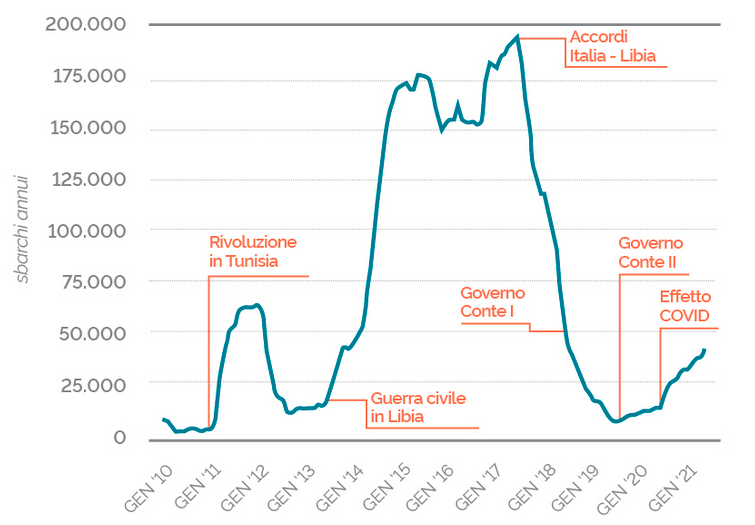
\includegraphics[width=0.8\columnwidth]{report/img/Sbarchi_15anni.png}
%    \caption{Refugees and migrants arriving in Italy by sea, from 2011 to 2021 with relevant events \cite{ispi} }
%    \label{fig:sbarchi}
%\end{figure}

As the number rose, Italy's far-right parties could frame the debate on migration in terms of "threats" and "security"\cite{iai}, making the issue a key element on their political platforms, as reported in some example tweets\cite{melonitweet}\cite{salvinitweet} of Figure \ref{fig:righttweet}. 

\begin{figure}[h]
\begin{subfigure}{.515\columnwidth}
  \centering
  
\includegraphics[width=\linewidth]{report/img/Meloni_tweet.png}
  \caption{Fratelli d'Italia’s tweet calling for a “naval blockade” to “protect Italy’s borders”}
  \label{fig:melonitweet}
\end{subfigure}%
\hfill
\begin{subfigure}{.4\columnwidth}
  \centering
  
\includegraphics[width=\linewidth]{report/img/Salvini_tweet.png}
  \caption{A tweet by Lega on keeping Italy “secure” from migrants}
  \label{fig:salvini tweet}
\end{subfigure}
\caption{Two example tweets of the electoral campaign of Summer 2022 by Fratelli d'Italia (Brothers of Italy) and Lega (League), that show the focus on "threat" and "security"}
\label{fig:righttweet}
\end{figure}

This resulted in echo-chambers that provided a distorted image of the real numbers about migrants and asylum seekers: according to a Ipsos study of 2019, the perceived presence of migrants on Italian territory is 31\% compared to the real data 9\%\cite{ipsos}. Furthermore, 63\% of Italians admitted that they were exposed to fake news on the theme Immigration, leading to believe that the majority of the crimes were committed by migrants (33 \% of the interviewed\cite{ipsos}), and that immigration establish a threat for Italy (57\% of the interviewed\cite{ipsos}).

As described in an article by Dylan Patrick Mcginnis on the Yale Review of International Studies\cite{salvinistrategy}, the Matteo Salvini's (leader of Lega) - and now Giorgia Meloni's (leader of Fratelli d'Italia) - strategy to put Immigration policy to the far-right relies mostly on creating an ‘us versus them’ dichotomy to ‘other’ migrants and on blaming immigrants for Italy’s poor economy.

According to these theses, the presence of a near conflict such as the Russian invasion of Ukraine, could let Italians empathize with the refugees; and that the similarity in terms of ethnicity could dismantle Salvini's 'us versus them' dichotomy.

In this paper it was therefore investigated the opinion dynamics of Italians about refugees, with a specific focus on the comparison and shift of opinions before and after the Russo-Ukrainian conflict of 2022.


\section{Data Collection}
For the goal of this paper, it was decided to create a new dataset. In fact, it was impossible to find a dataset which would fit our necessities. As described in this section, it was chosen to create two different datasets:
\begin{itemize}
    \item one used to build and analyze the graph;
    \item one used to train a classifier for the labelling of the tweets, regarding the Opinion Dynamics task.
\end{itemize}

\subsection{Selected Data Sources}

For the scraping of the data, it was chosen to use Twitter.
Twitter works as a public square for the public debate, in which politicians, journalists and everybody else can intervene for the creation of a discussion.
In particular, it was used the library snscraper\cite{snscraper}, which provides a simple scraping query in order to build a dataset based on the twitter data and metadata. 

\subsection{Crawling Methodology and Assumptions}

\subsubsection{Graph Creation}
Regarding the graph creation, it was decided to scrape all the tweets cointaining the hashtags \#rifugiato, \#rifugiati, \#profugo, \#profughi, \#migrante, \#migranti, in a temporal window from the first September 2020 until the first September 2022. As for the attributes, the following ones were scraped:
\begin{itemize}
    \item "User": username of the account writing the tweet;
    \item "Language": language of the tweet;
    \item "Date\_Tweet": date on which the tweet was written;
    \item "Tweet\_Id": number of identification of the tweet;
    \item "Tweet": actual content of the tweet;
    \item "Hashtags": list of hashtag in the tweet;
    \item "Conversation\_Id": number of identification of the conversation (all tweet replying to the same tweet have the same conversation id);
    \item "In\_reply\_To": account to which the tweet answer. If the tweet is the start of the conversation, this value is set to "User".
\end{itemize}

The first scraping produced 71735 tweets, for a total of 13575 unique Users and 69580 unique Conversations. These data had to be cleaned regarding the users subject to spam, i.e. the duplicated tweet from the same user were removed.
Also all the non-Italian written tweets were removed from the dataset.

Starting from the conversation id, a second scraping was performed, with the goal of reconstructing the whole conversation in which there is at least one tweet containing a keyword (i.e. a tweet that was already scraped). After the same spam elimination, it was decided to remove also the tweets of the people who were answering to themselves. 
After these cleaning procedures, in the dataset were left a total of 48262 unique Users. 

With these data, the graph was created. The users were chosen as nodes, while the replies between each user count as directed weighted link (based on the number of interactions between the users).
Using the graph visualizer \textit{Gephi}\cite{gephi}, it was observed that some source tweets of people acting as hubs were missing in the network, so another last scraping was necessary. 
Lastly the Users without any information, i.e. the users who were in the column "In\_reply\_To", but not the in the column "User", were eliminated. 

As a part of Data Understanding, it could be interesting to show how the number of tweets in our dataset change during the years, depicted in Figure \ref{fig:time}.

\begin{figure}[h]
    \centering
    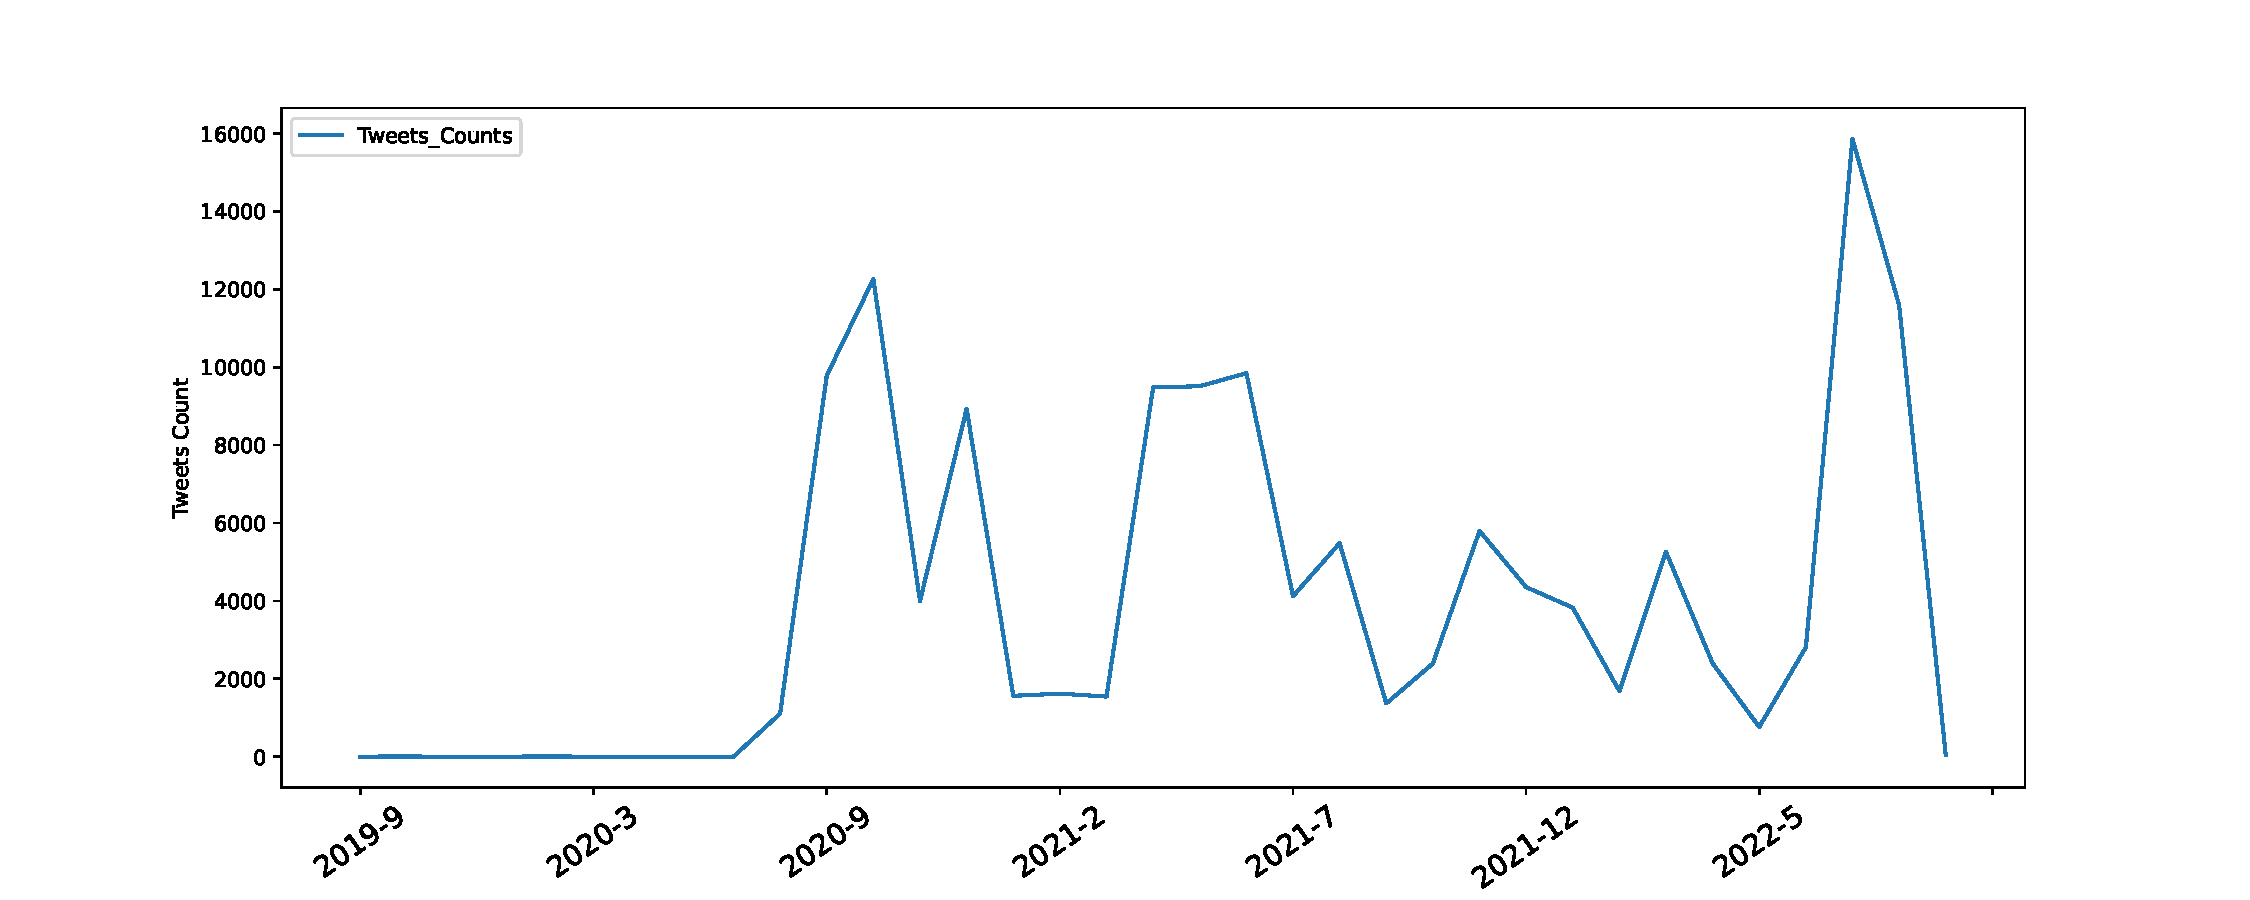
\includegraphics[width=\columnwidth]{report/img/tweets_time.pdf}
    \caption{Number of tweets vs time}
    \label{fig:time}
\end{figure}

One can notice how the counts of tweets have not an uniform distribution through time. This means that the topic of immigration is not always discussed, but rather has spars peaks correlated with news or source tweets by influencers. For example, the last peak is easily identifiable with the Italian electoral campaign of 2022, as immigration was one of the most discussed topics.

\subsubsection{Dataset for classification in the opinion dynamics}
In addition to the dataset used for the graph creation, it was chosen to create another one, in order to help with the opinion dynamics task. 
It was decided to scrape all the tweets from September 2018 to September 2022 written in Italian, containing the hastags \#portichiusi (closed harbors) and \#restiamoumani (stay human). The first was used by Matteo Salvini and other far right-wing people for an anti-immigration campaign\cite{portichiusi}, while the second was build by leftists and pro-immigration exponents as a response to \#portichiusi. The hashtag \#restiamoumani is also often associated with the international one \#RefugeesWelcome. 
On these tweets was applied a similar cleaning procedure to the first scraping. It was also noticed that out of the 131877 scraped tweets, only 808 regards the refugees from Ukraine.

In this new dataset, the label 1 was associated to the tweets containing only the hashtag \#restiamoumani, counting them as pro-refugees tweets. To the tweets containing only the hashtag \#portichiusi, the label 0 was associated, i.e. counting them as anti-refugees tweets. 

%\begin{figure}[h]
%    \centering
%    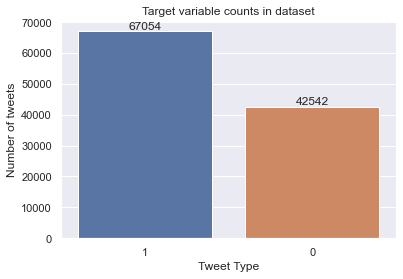
\includegraphics[width=0.8\columnwidth]{report/img/Classification_Train_Distribution.png}
%    \caption{Distribution of the classes in the Classification dataset}
%    \label{fig:class_dis}
%\end{figure}

\subsection{Nodes labeling}
The obtained dataset was used in order to train a classification model to label the original tweets; to do so, various different classification algorithms were tested. This dataset is slightly balanced towards a pro-refugees class, since the 1 label counts 67054 entries and the 0 label only 43542. When training the model, both oversampling and undersampling techniques were applied to improve the accuracy.
As a summary of the analysis the calibration plots  reported in Figure \ref{fig:calplot}. Logistic Regression Model gave the best performance, both in terms of accuracy (0.78) and in terms of probability calibration. 

\begin{figure}[h]
    \centering
    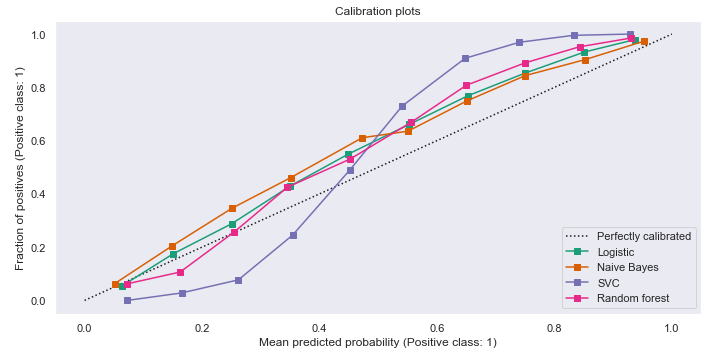
\includegraphics[width=0.8\columnwidth]{report/img/calibration_plot.png}
    \caption{Calibration Plots}
    \label{fig:calplot}
\end{figure}

Starting from binary tweet classification, the variable "user label" was created by assigning a continuous value to all users based on the number of positive tweets they wrote (labeled 1) out of the total number of tweets. Basically, the closer the obtained mean is to 1, the more positive the user's opinion is (pro-refugee) and vice versa. 

\section{Network Characterization}

As described in the previous section, the network from Real World (RW) is composed by the User acting as nodes and tweet replies as weighted links. In order to create this graph, it was decided to use the library \textit{NetworkX}\cite{SciPyProceedings_11}. Visualizing the graph in \textit{Gephi}, it was noticed the abundant presence of isolated nodes, which were considered not interesting for the analysis. Also, some algorithms used to characterize the network are computationally expensive. For this reason, it was decided to work only with the giant component and to render the graph undirected and unweighted for this task.
At the end of the cleaning one counts 46978 nodes and 88029 links. 
Our RW network has a density of $7.98\cdot 10^{-05}$, an average Clustering Coefficient of 0.078 and an average shortest path of 3.39. The nodes acting as hubs are 93, while the Degree and Clustering Coefficient distributions can be seen in Figures \ref{fig:degree_RW} and \ref{fig:cc_dis}.

\begin{figure}[h]
    \centering
    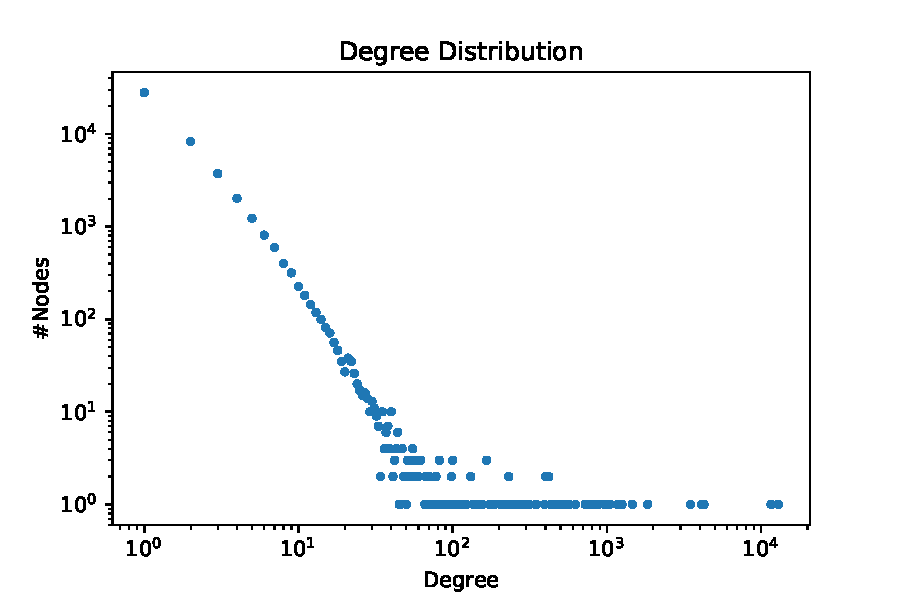
\includegraphics[width=0.9\columnwidth]{report/img/degree_distribution.pdf}
    \caption{Degree Distribution of RW Network}
    \label{fig:degree_RW}
\end{figure}

\begin{figure}[h]
    \centering
    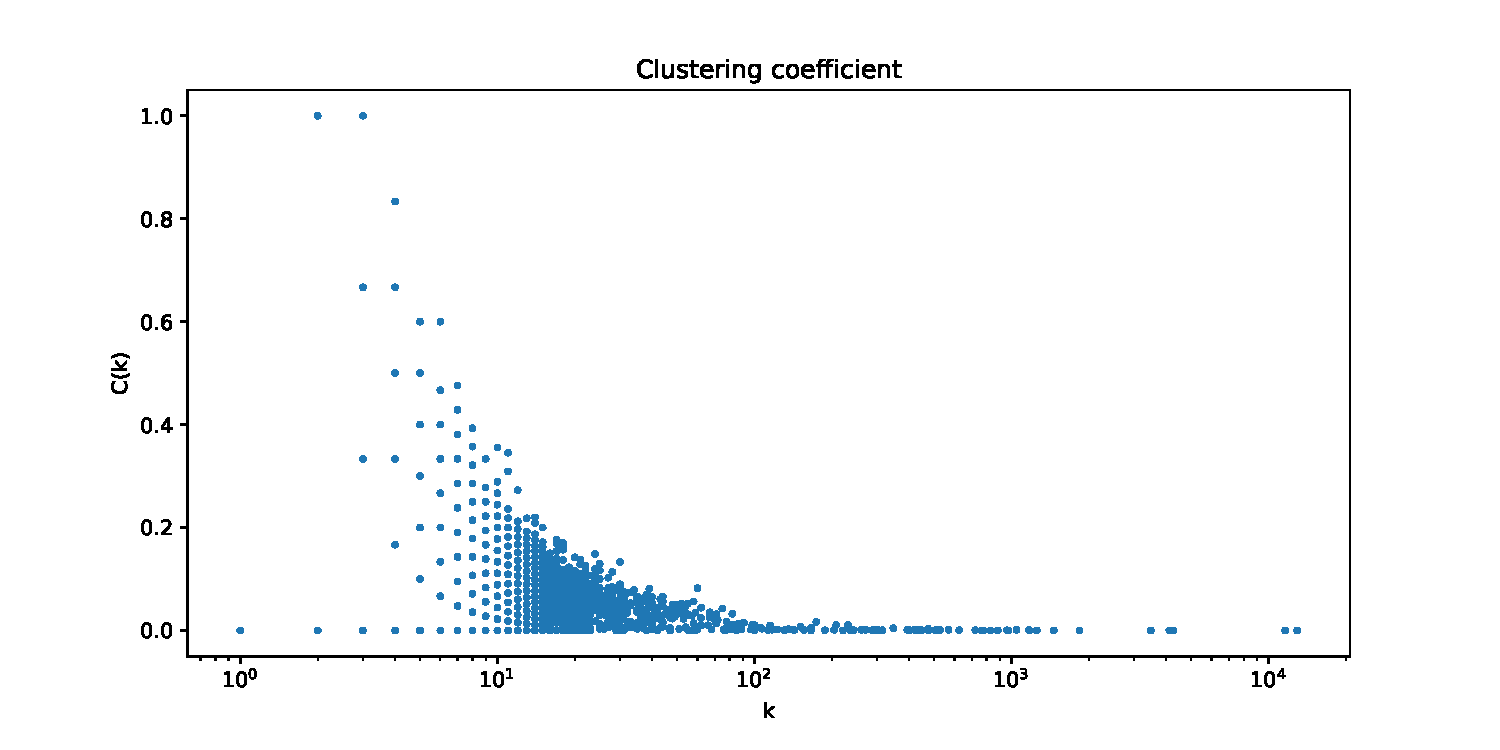
\includegraphics[width=0.9\columnwidth]{report/img/cluster_coefficient_distribution.pdf}
    \caption{Clustering Coefficient Distribution of RW Netork with respect to the degree \textit{k}}
    \label{fig:cc_dis}
\end{figure}


The Centrality Analysis was performed using different measures, in particular: Degree, Betweenness, Closeness, Harmonic, PageRank and Eigenvector. The Degree, PageRank and Eigenvector Centrality produces similar results. Between these three it was chosen to show the Degree Centrality, depicted in Figure \ref{fig:degree_centrality}. As one can see, the most important nodes for this measure are Matteo Salvini (Lega) and Giorgia Meloni (Fratelli d'Italia). It follows a list of public figures, like other politicians (Giuseppe Conte, Enrico Letta, Luigi Di Maio) and journalists (Corrado Formigli, Roberto Saviano).

\begin{figure}[h]
    \centering
    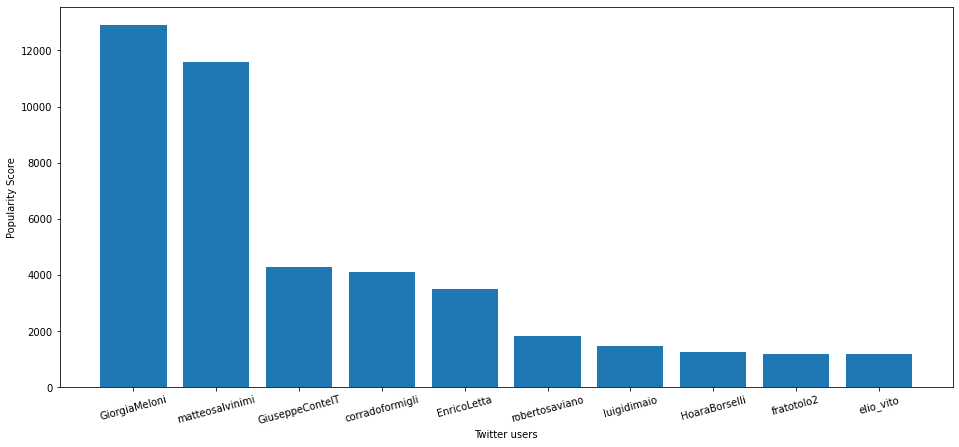
\includegraphics[width=0.8\columnwidth]{report/img/Degree_centrality.png}
    \caption{Degree Centrality}
    \label{fig:degree_centrality}
\end{figure}

More interesting is the bar plot of the Harmonic Centrality, that can be seen in Figure \ref{fig:closeness_centrality}. In this plot, one can see that private users can be almost as central as public figures. 

\begin{figure}[h]
    \centering
    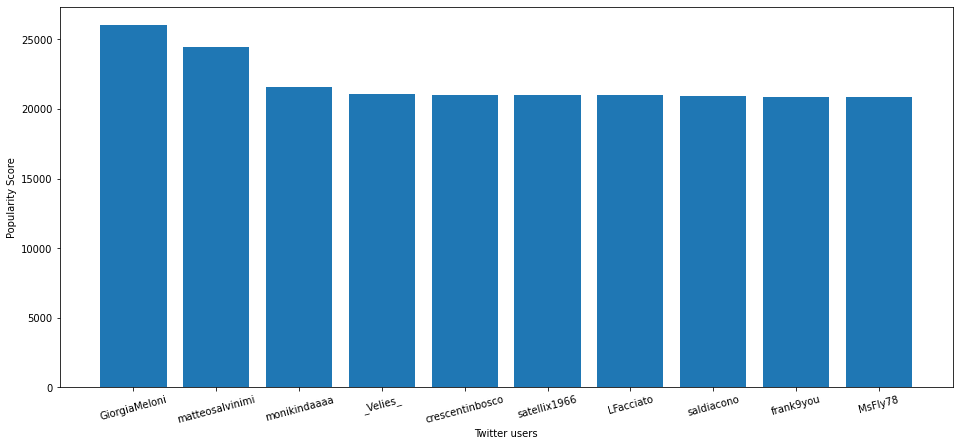
\includegraphics[width=0.8\columnwidth]{report/img/Harmonic_centrality.png}
    \caption{Closeness Centrality}
    \label{fig:closeness_centrality}
\end{figure}

To measure the homophily of the graph, it was used the assortativity measure $R$ implemented by the library \textit{NetworkX}, which uses the Pearson correlation coefficient between pairs of linked nodes' degrees. For this reason, the assortativity may also be considered a correlation measure between nodes. 

Our RW network is classified as slightly disassortative, because of $R=-0.2$. This can be explained by the behaviour of small nodes that tend to connect with a greater probability with hubs, and not with other small nodes. This effect can also be seen in Figure \ref{fig:assortativity}, which depicts the distribution of the average nearest neighbor degree of nodes with degree k.

\begin{figure}[h]
    \centering
    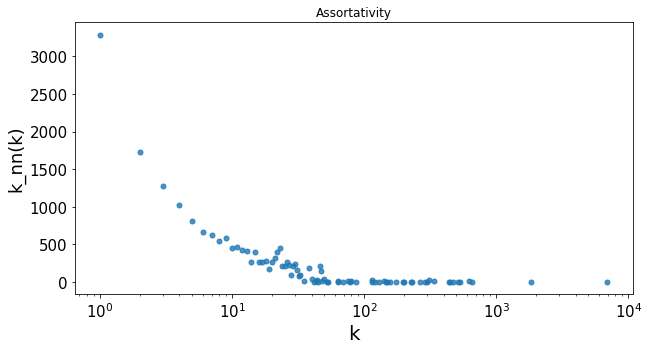
\includegraphics[width=\columnwidth]{report/img/Assortativity_distribution.png}
    \caption{Assortativity Distribution with respect to the degree \textit{k}}
    \label{fig:assortativity}
\end{figure}

\subsection{Comparision with Erdős–Rényi, Barabási-Albert, Watts-Strogatz Models}

In order to compare the RW network with the theory models, three synthetic graphs were generated, in particular:
\begin{itemize}
    \item Erdős–Rényi (ER) Graph\cite{erdos}: in order to obtain a similar number of Nodes and Edges, it was set N=46978 and p=0.0000787, for a total number of edges of E=86768;
    \item Barabási-Albert (BA) Graph\cite{barabasi}: as above, it was set N=46978 and m=2, making E=93952;
    \item Watts-Strogatz (WS) Graph\cite{watts}: N=46978, k=4, p=0.8, leading to E=93956.
\end{itemize}

The other basic characteristics such as Average Degree (Degree) Connected Components (CC), Density, Average Clustering Coefficient (AClCo), Average Path Length (APL) of the simulated networks are summarized in Table \ref{tab:proper}. 

\begin{table}[h]
    \centering
        \caption{Characterization of RW and Simulated Networks. It shows number of Nodes, number of Edges, Average Degree (Degree), Density, Average Clustering Coefficient (AClCo) and Average Path Length (APL).}
     \adjustbox{max width=\columnwidth}{%
    \begin{tabular}{c|c|c|c|c|c|c|c}
    
         &  Nodes & Edges & Degree & CC & Density & AClCo & APL\\\hline
         
         RW & 46978 & 88029 & 3.75 & 1 & $7.98\cdot 10^{-5}$ & 0.078 & 3.39\\
         
         ER & 46978 & 86768 & 3.69 & 1214 & $7.86 \cdot 10^{-5}$ & $5.93 \cdot 10^{-5}$ & 1.66\\
         
         BA & 46978 & 93952 & 3.99 & 1 & $8.51 \cdot 10^{-5}$ & 0.0014 & 9.21\\
         
         WS & 46978 & 93956 & 4.0 & 1 & $8.51 \cdot 10^{-5}$ & 0.0044 & 2.38
    \end{tabular}
    }
    \label{tab:proper}
\end{table}

Comparing the degree distribution in Figure \ref{fig:degree_distribution_comparison}, one can notice how the RW and the BA model follow a similar shape. This behaviour is explained by the nature of the BA model itself, since it reproduces preferential attachment and hubs, which play a very important role in the Real World Networks. 
The degree distribution of ER and WS are both Poissonian and tend to go to zero quickly, as well depicted in Figure \ref{fig:degree_distribution_comparison}.

\begin{figure}[h]
    \centering
    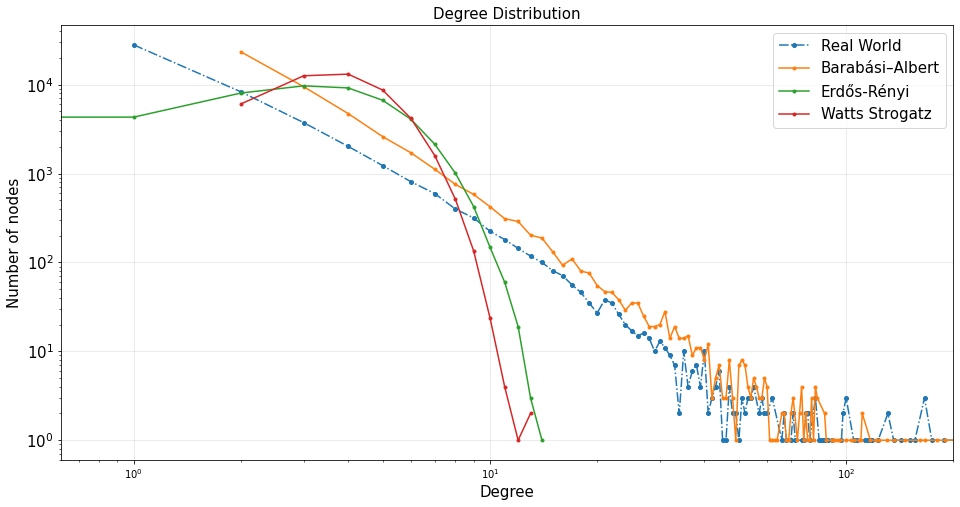
\includegraphics[width=0.8\columnwidth]{report/img/Degree_distribution_comparison.png}
    \caption{Degree Distribution Comparison}
    \label{fig:degree_distribution_comparison}
\end{figure}

Regarding the path analysis, the algorithms are very expensive in terms of time of execution. For this reason, it was decided to build a sampled graph of the ER network of 15000 nodes and focus only on the giant component. In order to speed up the analysis, the results may then result biased by this choice.

\section{Task 1: Community Discovery}

Through discussion or searching information, people are influenced by their neighbours and by the environment around them. For that reason, studying how users were distributed among communities during the two years of observation is useful to understand the evolution of the network. 
Defining what a community is and how it born is not a trivial task. This section will show different ways to detect them based on different strategies.
Two different kinds of community discovery methods were run:

\begin{itemize}
    \item the first one refers to a static view of graph where the network is not supposed to be influenced by the time dimension;
    \item the second one is instead considered dynamic for the opposite reason. Few snapshots will be used in order to achieve this goal.
\end{itemize}

In both cases, the graph links were considered undirected and weighted because most of the algorithms do not support directed links.

\subsection{Community evaluation’s formulas}
During the evaluation phase internal and external evaluation was made using CDLib modules. In order to uniquely identify formulas used in this process, a brief description is given:

\begin{itemize}
    \item \textit{Internal evaluation:} fitness functions allow to summarize the characteristics of a computed set of communities.
    \begin{itemize}
        \item \textbf{Conductance:} it is the fraction of total edge volume that points outside the community. Lower values are preferable than higher.
        \begin{equation}
            f(S)=\frac{c_S}{2m_S+c_S}
        \end{equation}
        \item \textbf{Newman-Girvan Modularity:}\cite{ngmod} it is the difference of the fraction of intra community edges of a partition with the expected number of such edges if distributed according to a null model.  In other terms, modularity compares the real network structure with a corresponding one where nodes are connected without any preference about their neighbours. The aim is to maximize it. 
        \begin{equation}
            Q(S)=\frac{1}{m}\sum_{c \in S}\biggl(m_S-\frac{(2m_S+l_S)^2}{4m}\biggr)
        \end{equation}
    \end{itemize}
 
    \item \textit{External evaluation:} it is useful to compare different graph partition to assess their resemblance.
    \begin{itemize}
        \item \textbf{Adjusted Mutual Information:} it is an adjustment of the Mutual Information. It accounts for the fact that the MI is generally higher for two clustering with a larger number of clusters, regardless of whether there is actually more information shared.
        \begin{equation}
            AMI(U,V)=\frac{MI(U,V)-E(MI(U,V))}{\max(H(U),H,V)-E(MI(U,V))}
        \end{equation}
 
        where U and V are clusters;
        \item \textbf{Overlapping Normalized Mutual Information LFK:} it is an extension of the Normalized Mutual Information (NMI) score to cope with overlapping partitions. Higher values are preferable than lower ones. It is a variant implemented by Lancichinetti \cite{Lancichinetti_2009}

        \item \textbf{Normalized F1 Score:} it computes a score of the optimal algorithms matches among the partitions in input. It works on overlapping/non-overlapping complete/partial coverage partitions. Higher values are preferable than lower ones\cite{inproceedings}. 
        %REFERENCE Rossetti, G., Pappalardo, L., & Rinzivillo, S. (2016). A novel approach to evaluate algorithms detection internal on ground truth.
    \end{itemize}    
    \item The last measure implemented was \textbf{Jaccard} computed as: 
    \begin{equation}
        J(U,V)=\frac{\vline U \cup V \vline}{\vline U \cap V\vline}
    \end{equation}
\end{itemize}

\subsection{Static community discovery}
The algorithms used in this section – using CDLib\cite{cdlib} modules - regards three different ways of constructing communities:
\begin{itemize}
    \item Crisp communities: nodes belong to only one community (Label propagation\cite{Raghavan_2007}, Louvain\cite{Blondel_2008}, Leiden\cite{louvain} was implemented)
    \item Overlapping communities: nodes can belong to different communities simultaneously   (Demon\cite{demon}, Angel\cite{angel}, K-clique were implemented)
    \item Fuzzy communities: each node has assigned a probability to belong in a community. (Principled clustering was implemented)
\end{itemize}

During the hyperparameter tuning phase a grid search was run for those algorithms that have a specific metric to maximize or minimize. For the others a script was implemented in order to compare conductance and \textit{Newman-Girvan modularity} and choose the best trade-off between them. Table \ref{tab:cd} shows the result of the most informative metrics used to evaluate communities obtained during the analysis.

\begin{table*}[h]
    \centering
        \caption{Summary of parameters, results and performance of the algorithms used for community discovery}
    %\adjustbox{max width=\columnwidth}{%
    \begin{tabular}{c|c|c|c|c|c}
         &  Parameter(s) & $\#$Communities & Node coverage & Conductance & NG Modularity\\\hline\hline
         \textbf{Label propagation} &	none&	1781&	1&	0.8461&	0.4550\\
\textbf{Louvain} &	resolution= 0.9 &	31&	1&	0.375&	0.5874\\
\textbf{Leiden} &	none &	40 &	1&	0.3761&	0.5952\\
\textbf{Demon} &	$\varepsilon= 0.1$, min$\_$com$\_$size= 3 &	18 &	0.1694 &	0.9854 &	0.05\\
\textbf{Angel}	& t= 0.1, min$\_$com$\_$size= 6 &	3 &	0.1054 &	0.8788 &	0.2507\\
\textbf{K-Clique} &	K= 3 &	912 &	0.1926 &	0.9237 &	0.0141\\
\textbf{Principled Clustering} &	num$\_$communities= 4 &	4	& 1 &	0.2972 &	0.4491

    \end{tabular}
    %}

    \label{tab:cd}
\end{table*}

Based on the table, Louvain, Leiden and principled clustering performed better than other in both the metrics.

 Interesting for the analysis is a comparison between the different communities returned, in order to assess if they are matching or not. The way in which the comparison was done takes in consideration the adjusted mutual information for communities that do not overlap and the overlapping normalized mutual information for communities that overlap. This analysis was done knowing that the results may be biased because some algorithms optimize different metrics. For this reason, it was difficult to compare the algorithms in terms of efficiency. The most significant similarities - excluding the one between Louvain and Leiden which was predictable - were between the non overlapping communities. In Figure \ref{fig:cd} is visualized the comparison of them using an heatmap. 
 
 \begin{figure}[h]
     \centering
     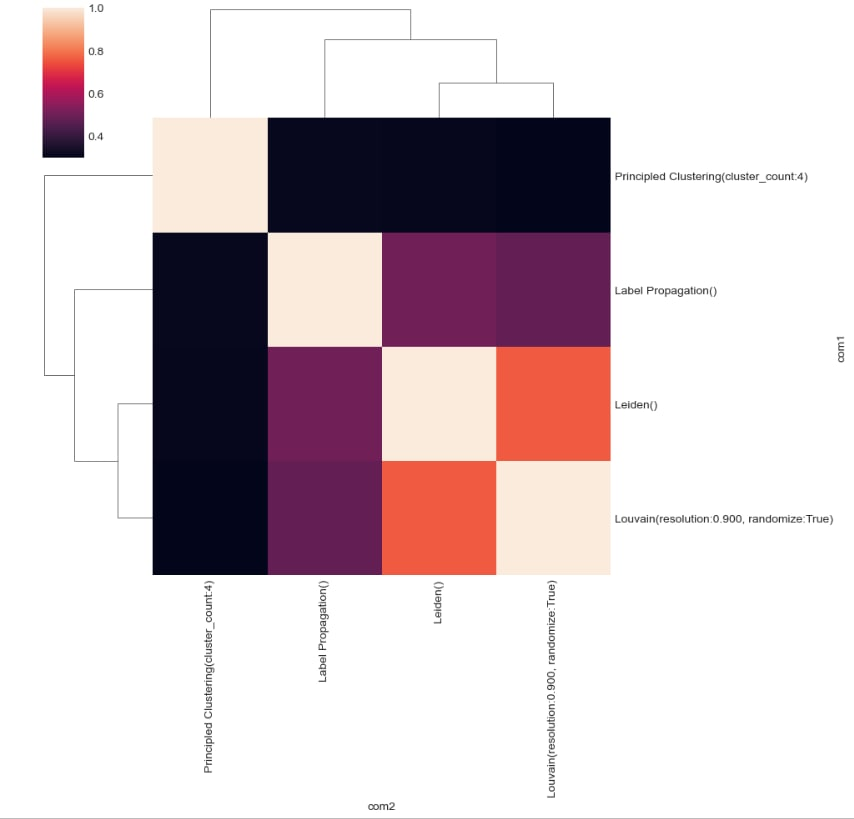
\includegraphics[width=0.75\columnwidth]{report/img/heatmap.jpeg}
     \caption{Heatmap of different Community Discovery algorithms used}
     \label{fig:cd}
 \end{figure}
 
This static analysis has the advantage of being easier to implement but has a lot of limitation as the impossibility to detect community events. In real networks, communities change or evolve at every timestamp and identifying their transformation is helpful also to understand how users change their opinions, friendship etc. To achieve this goal, a dynamic community discovery is implemented.

\subsection{Dynamic Community Discovery}

For the task of dynamic community discovery, it was decided to divide the dataset in semesters and then the giant component was extracted for each of them. In order to be coherent during the split, all the tweets related to a conversation started in the given semester are also considered inserted in that semester. 
The number of tweets in each semester are respectively 17440, 17387, 10090, 18205 denoting a uniform distribution, except for the third period. Being aware of the results reached in the static analysis, the algorithms selected for this task were Leiden and Principled Clustering. The idea was to treat the different semester as a static snapshot and perform on it the selected community discovery’s algorithm. The purpose was to evaluate whether there were matches between the created temporal clusters and investigate the communities life events occurred in the meanwhile.
As for the static analysis an hyperparameter tuning was needed for Principled Clustering in order to choose the best trade-off between conductance and modularity. In Table \ref{tab:cddin} are returned the parameter configuration and the results given by the comparison between communities of adjacent snapshots in terms of stability using Normalized F1 score.

\begin{table}[h]
    \centering
        \caption{Results and performance of Leiden and Principled Clustering (PC) on the four different snapshots}
    \adjustbox{max width=\columnwidth}{%

    \begin{tabular}{c|c|c|c|c}
         Snapshot & \multicolumn{2}{|c|}{\# Communities} &\multicolumn{2}{|c}{ Normalized F1 Score} \\\cline{2-5}
         & Leiden & PC & Leiden & PC\\\hline\hline
         Sep 2020 – Feb 2021 & 60 & 8 & - & -\\
        Mar 2021 – Aug 2021 & 38  & 9 & 0.001914 & 0.007343\\
        Sep 2021 – Feb 2022 & 46  & 8 & 0.000493 & 0.016666\\
        Mar 2022 – Aug 2022 & 35 & 9 & 0.001925 & 0.010277\\

         & 
    \end{tabular}
    }

    \label{tab:cddin}
\end{table}

As it is evident from the data, principled clustering performs better in terms of stability although results are below the expectation. Low stability could be explained by making a deeper analysis on communities’ composition and on snapshot composition. Using Jaccard as a metric, it was investigated how many users that were present in a snapshot were also present in the following one, and how many users that were present in the first snapshot were also available in the last one. Data showed that on average only 13$\%$ of the users are shared between snapshots, while the others are totally new ones. This inhomogeneous conformation could create a great difficulty in detecting stable communities. With the aim to investigate communities life events a Sankey Plot was constructed, regarding a sample of matching communities returned by principled clustering. According to Wikipedia, Sankey diagrams are a type of flow diagram in which the width of the arrows is proportional to the flow rate\cite{sankey}. As one can see in Figure \ref{fig:alluvial} different events are present like born and merges.

\begin{figure}[h]
    \centering
    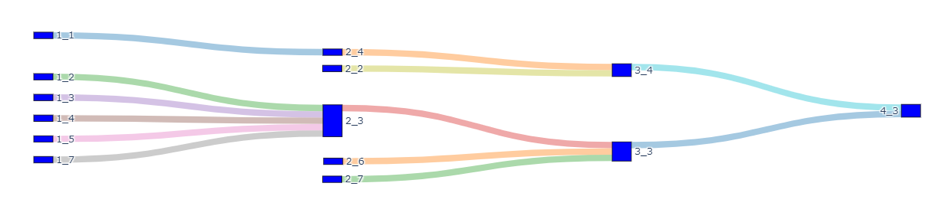
\includegraphics[width=\columnwidth]{report/img/alluvial_cd.png}
    \caption{Sankey plot of the communities life through time}
    \label{fig:alluvial}
\end{figure}

With the aim to improve the stability of clusters it was chosen Tiles \cite{tiles}.
%REFERENCE Rossetti, Giulio; Pappalardo, Luca; Pedreschi, Dino, and Giannotti, Fosca. `Tiles: an online algorithm for community discovery in dynamic social networks.<https://link.springer.com/article/10.1007/s10994-016-5582-8>`_ Machine Learning (2016), 106(8), 1213-1241. 
 Tiles is based on an online method which does not partition the full temporal graph, but tries to build and maintain communities in an online fashion following the rising and vanishing of new nodes and edges. In this way, communities’ changes were evaluated each time using a few numbers of new users giving a smooth evolution of clusters. As before, four snapshots were used to create the dynamic network. The results achieved are given Table \ref{tab:tiles}.

\begin{table}[h]
    \centering
        \caption{Summary of Tiles}
    \begin{tabular}{c|c|c}
         Snapshot & $\#$communities & Stability trend  \\\hline
        Sep 2020 – Feb 2021 &	587	 &     -  \\
        Mar 2021 – Aug 2021 &	1040 &	0.1445\\
        Sep 2021 – Feb 2022 &	1254 &	0.2171\\
        Mar 2022 – Aug 2022 &	1627 &	0.2106\\

    \end{tabular}

    \label{tab:tiles}
\end{table}

As expected, Tiles produces communities that are more stable than other algorithms; the main problem is represented by the huge number of communities created that make their representation and analysis very complex.
For the next task, when communities discovered are involved, they are considered as those created by the principled clustering algorithms despite being aware of problems related to non-deterministic ones. This decision was principally taken due to the possibility of better managing them when a qualitative analysis on users were needed.

Lastly, it could be interesting to study how the user label distributed in each community through time. As shown in Figure \ref{fig:community_distribution_5}, one can see that a community does not really represent a definite opinion. This behaviour is similar to all the distributions, and it is confirmed by the high variance and similar mean of each distribution. This is not surprising, since the communities are built by topological assumption and not by taking in consideration the user label. This may be a hint that a community represents a topic, i.e. users with different opinions interact with each others over a defined topic. Moreover, it can be noticed in Figure \ref{fig:community_distribution_5} that the user label distribution appears to be stable through time, i.e. the changes of the bins are small.

\begin{figure}[h]
\centering

\begin{minipage}[b]{.48\linewidth}
\centering\large 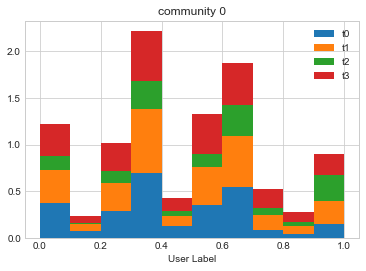
\includegraphics[width=0.9\linewidth]{report/img/community_distribution_0.png}
\subcaption{Community 0}
\end{minipage}%
\begin{minipage}[b]{.48\linewidth}
\centering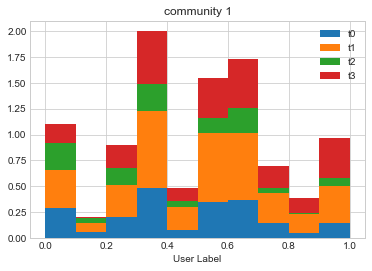
\includegraphics[width=0.9\linewidth]{report/img/community_distribution_1.png}\subcaption{Community 1}
\end{minipage}

\begin{minipage}[b]{.48\linewidth}
\centering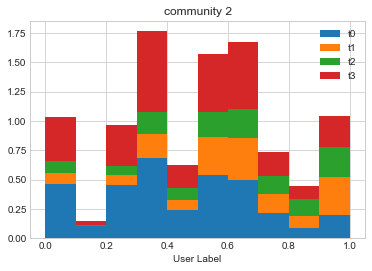
\includegraphics[width=0.9\linewidth]{report/img/community_distribution_2.png}\subcaption{Community 2}\label{fig:famdis}
\end{minipage}
\begin{minipage}[b]{.48\linewidth}
\centering\large 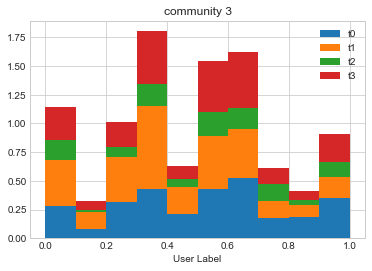
\includegraphics[width=0.9\linewidth]{report/img/community_distribution_3.png}
\subcaption{Community 3}
\end{minipage}%

\begin{minipage}[b]{.48\linewidth}
\centering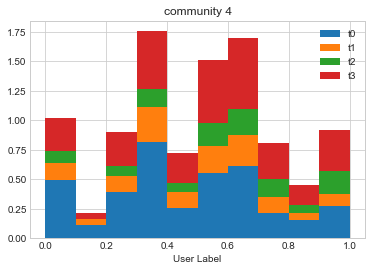
\includegraphics[width=0.9\linewidth]{report/img/community_distribution_4.png}\subcaption{Community 4}
\end{minipage}
\begin{minipage}[b]{.48\linewidth}
\centering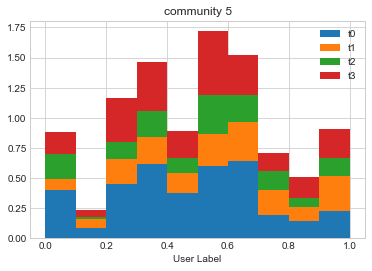
\includegraphics[width=0.9\linewidth]{report/img/community_distribution_5.png}\subcaption{Community 5}
\end{minipage}

\begin{minipage}[b]{.48\linewidth}
\centering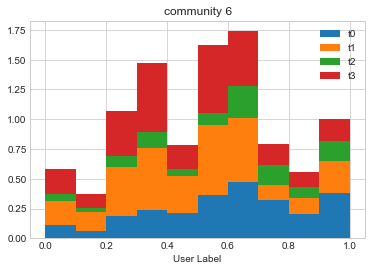
\includegraphics[width=0.9\linewidth]{report/img/community_distribution_6.png}\subcaption{Community 6}
\end{minipage}
\begin{minipage}[b]{.48\linewidth}
\centering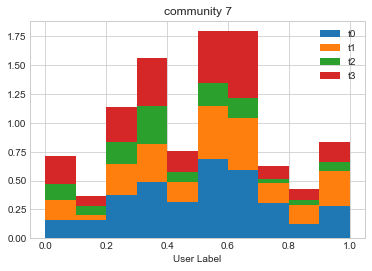
\includegraphics[width=0.9\linewidth]{report/img/community_distribution_7.png}\subcaption{Community 7}
\end{minipage}

    \caption{Distribution of user label for the communities in the all timestamps}
    \label{fig:community_distribution_5}

\end{figure}




%\begin{figure}[h]
%    \centering
%    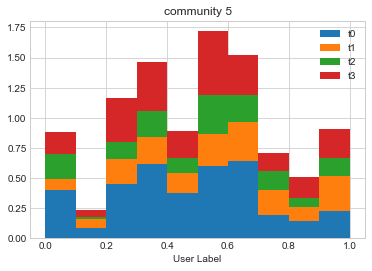
\includegraphics[width=0.8\columnwidth]{report/img/community_distribution_5.png}
%    \caption{Distribution of user label for the community 5 in the all timestamps}
%    \label{fig:community_distribution_5}
%\end{figure}

\section{Task 2: Opinion Dynamics}

In this section some Opinion Dynamics models have been explored, in order to shape the way the opinions about refugees spread in the network. For this purpose, three discrete models were implemented from \textit{NDlib} python library\cite{ndlib}: \textit{Voter Model}\cite{voter}, \textit{Majority Rule}\cite{Galam_2002} and \textit{Sznajd Model}\cite{SZNAJD_WERON_2000}. These models were ran on the strongly connected component of the graph, with 46978 nodes. Visualizing the network on \textit{Gephi}, it was noticed that 50\% of the users had an opinion between 0.5 and 1 and the remaining 50\% had an opinion between 0 and 0.5; the results were then compared with those of two synthetic models (the \textit{Barabási-Albert} and the \textit{Watts-Strogatz} networks), by applying the same algorithms and parameters. 
Although opinions in the network are expressed continuously, for this task it was decided to run only discrete models of opinion dynamics in order to have simpler results to read and interpret. A more detailed analysis of how real user opinion changes over time is presented in the open-question section. 

\subsection{Voter Model}
The \textit{Voter} model is one of the simplest models of opinion dynamics. It is possible to imagine that each node in the graph has a discrete opinion (±1). At each timestamp the opinion of a random node \textit{i} is changed (or confirmed) with the opinion of a neighboring node \textit{j} -also taken randomly. In our context, the model was run for 2000 iterations on the RW graph, starting from a perfectly balanced situation between infected and susceptible nodes (fraction 0.5).The results were then compared with those obtained from the same model with the same parameters applied to the synthetic graphs. 

The \textit{Voter} model in the RW shows a fluctuating initial condition, until, as the iterations grow up, fluctuations tend to decrease. 
The same exact behavior is not observed in either of the two synthetic graphs, although the BA graph approaches the RW network trend, even if with the opposite opinion, as shown in Figure \ref{fig:Voter}.

\begin{figure}[h]
\centering
\begin{subfigure}[H]{1\columnwidth}
    \centering
   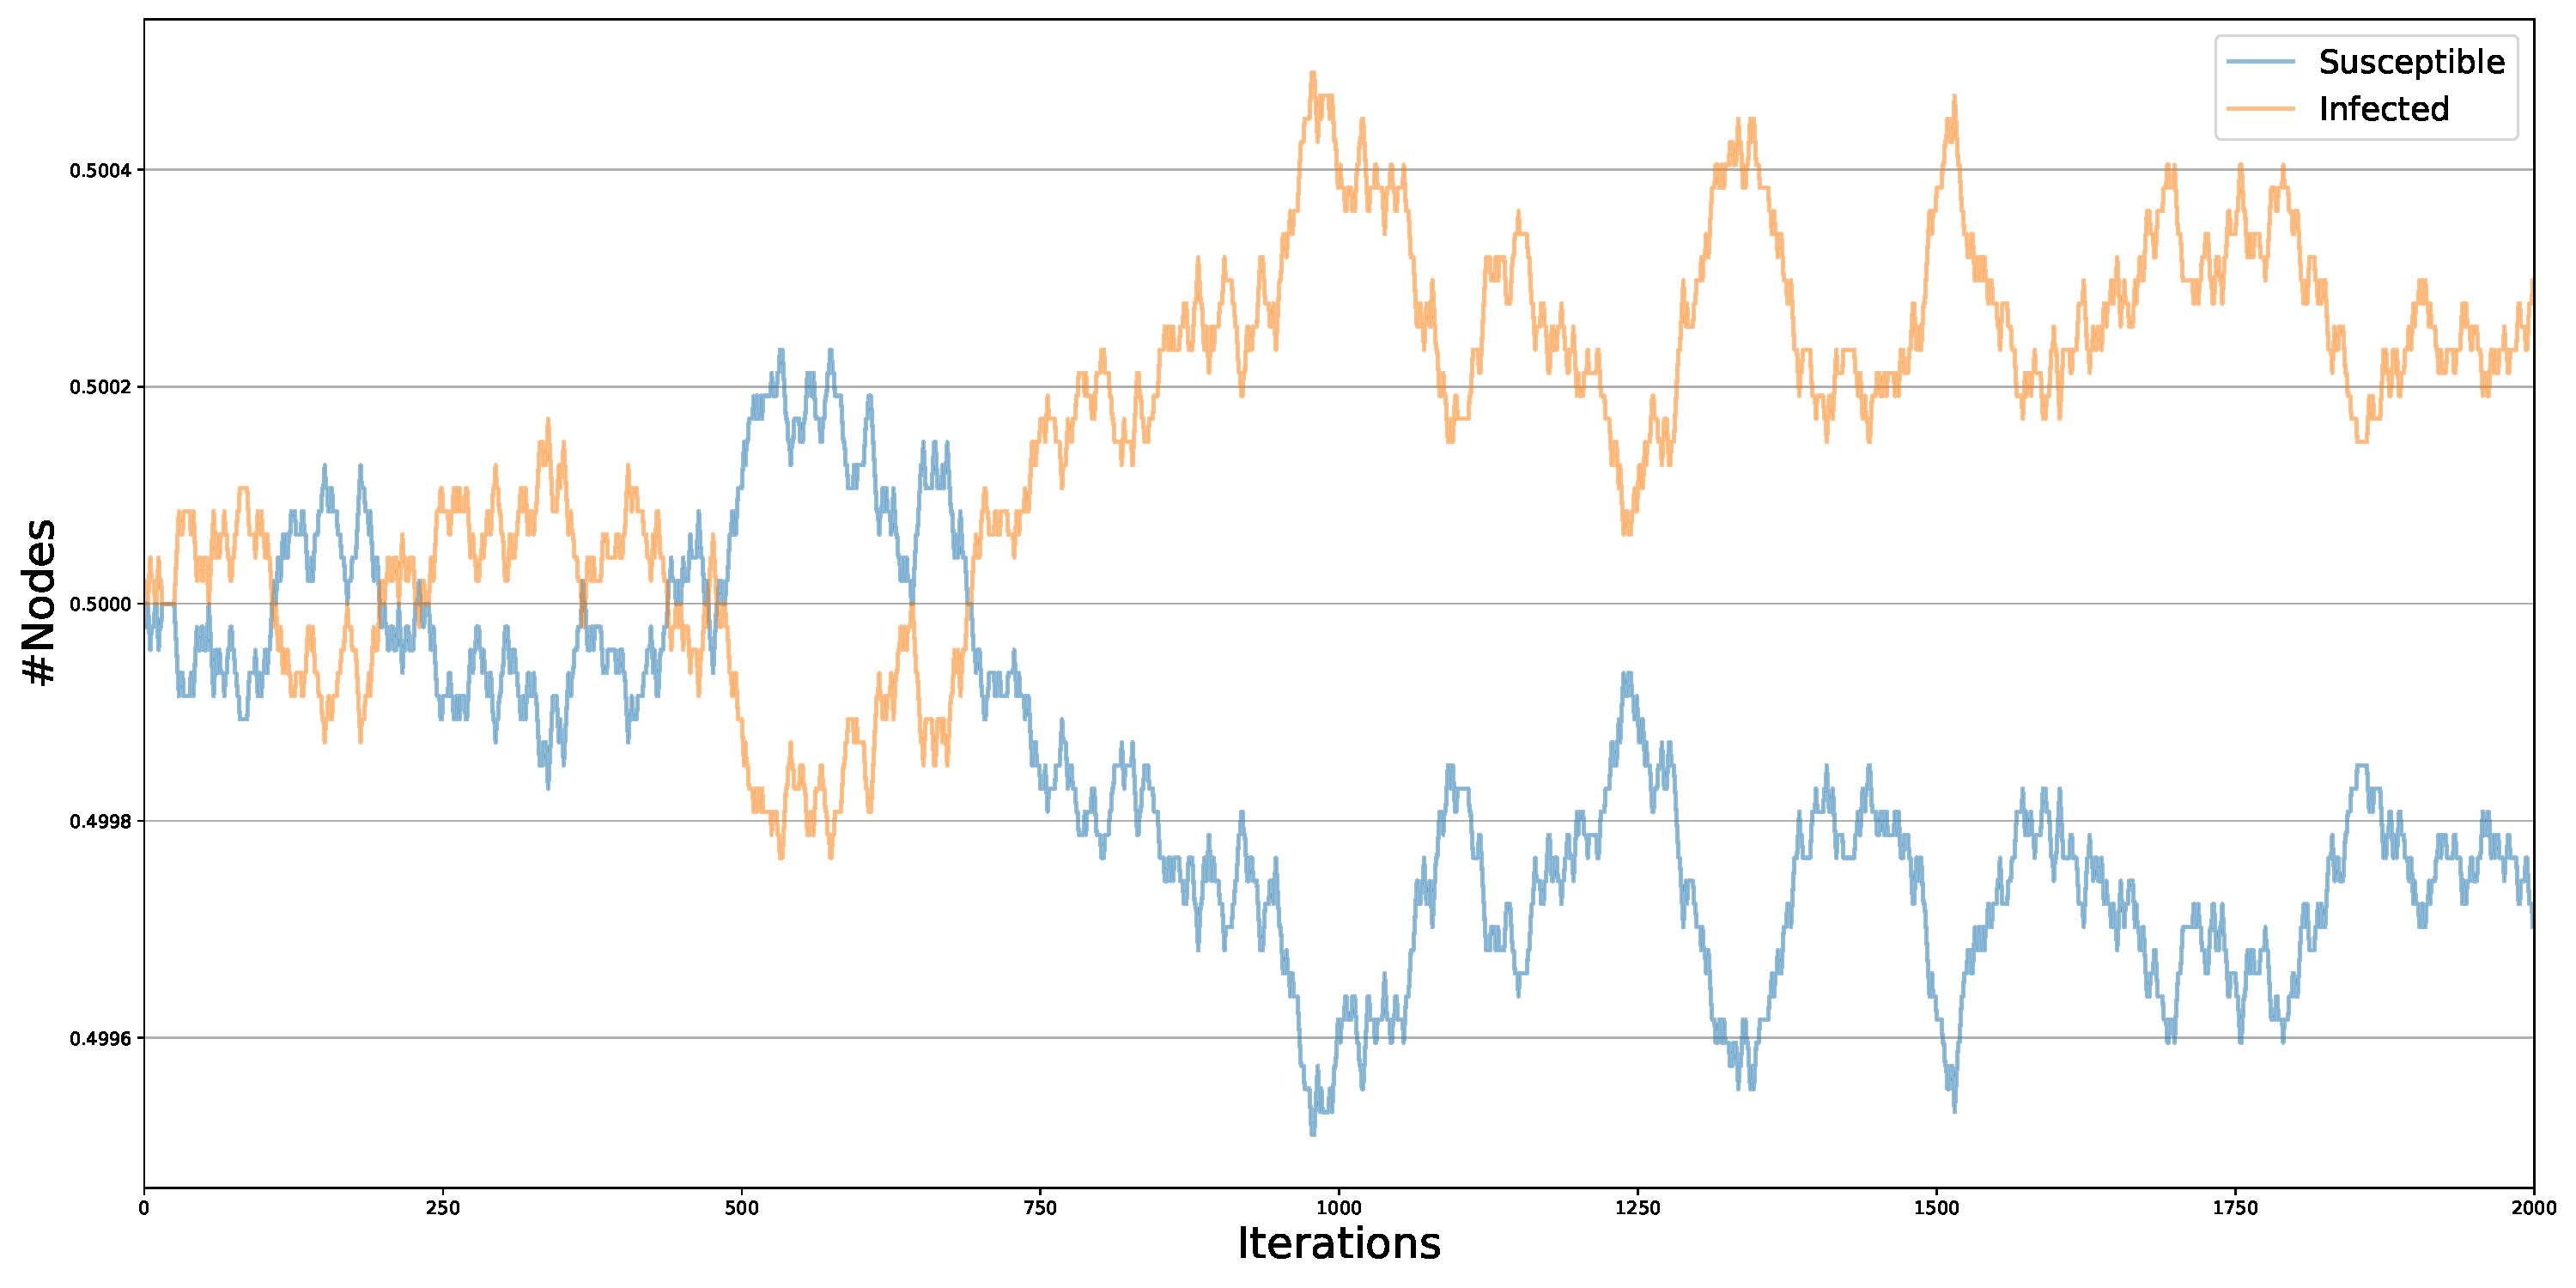
\includegraphics[width=.9\linewidth]{report/img/OD/Voter_0.5.pdf}
   \caption{Real World Network}
   \label{fig:RW_Voter} 
\end{subfigure}

\begin{subfigure}[H]{1\columnwidth}
   \centering
   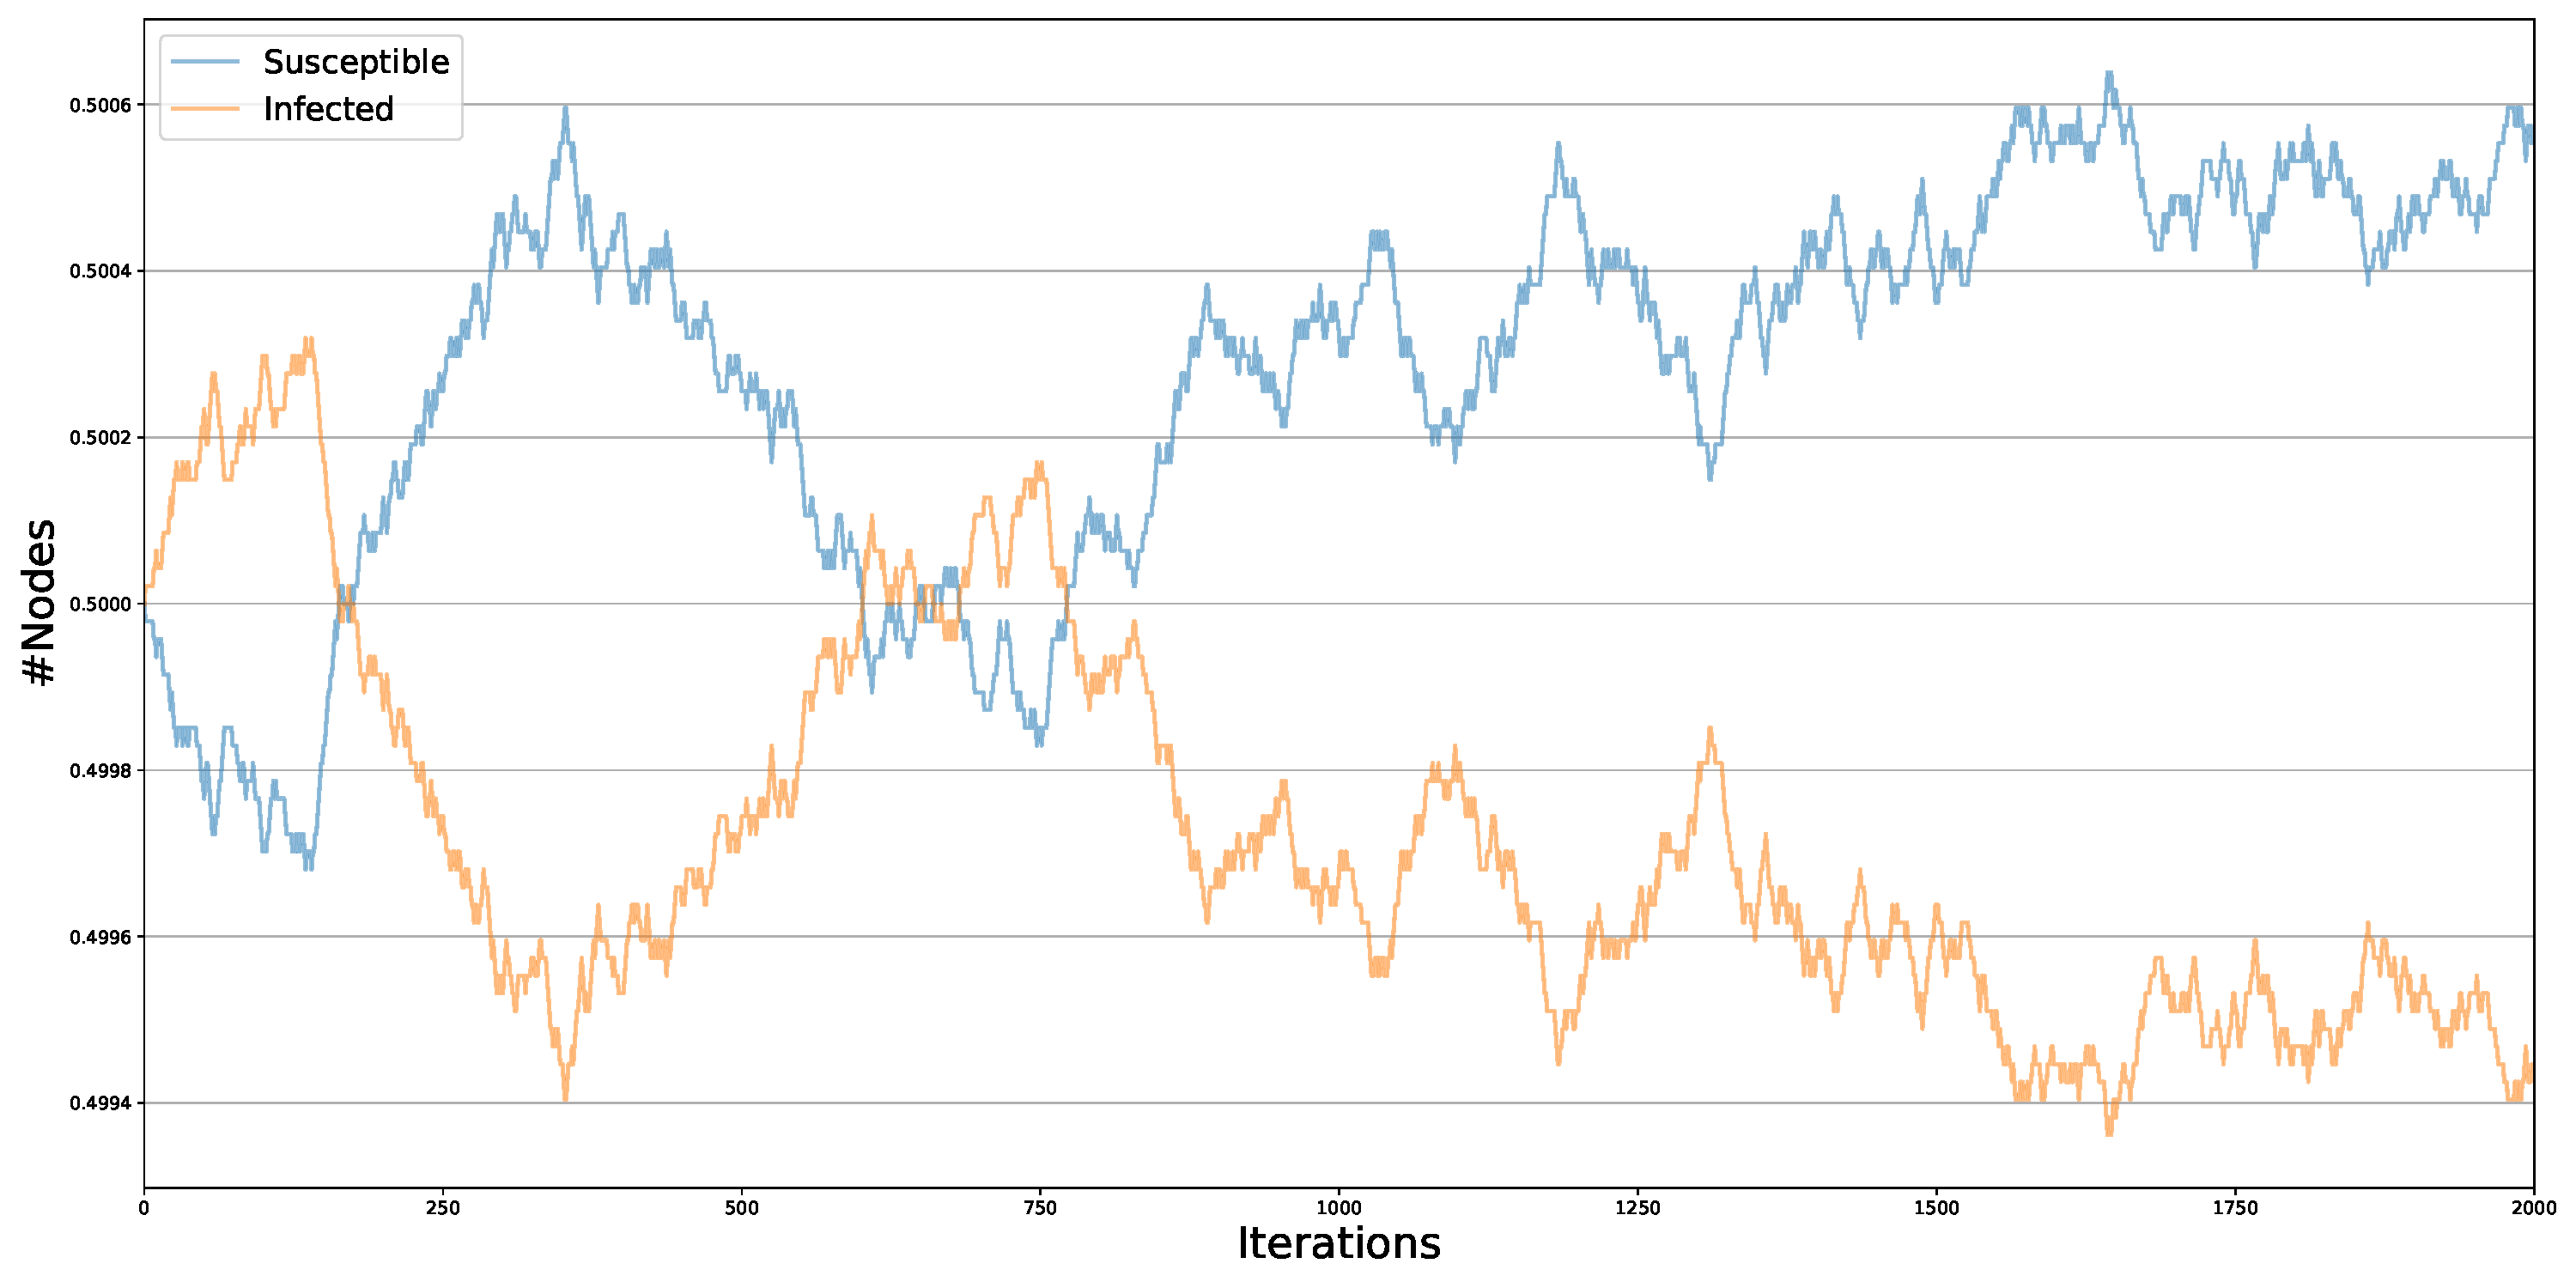
\includegraphics[width=.9\linewidth]{report/img/OD/VoterBA_0.5.pdf}
   \caption{Barabasi-Albert Network}
   \label{fig:BA_Voter}
\end{subfigure}

\caption{Voter Model}
\label{fig:Voter}
\end{figure}

\subsection{Majority Rule model}
The \textit{Majority Rule} model is one of the discrete opinion's model, in which each agent has a discrete opinion ±1. The difference with \textit{Voter} lies on \textit{social inertia} concept: i.e., an individual's hostility to change its social group. The model, starting from a random group of nodes with their opinion, assigns each node the majority opinion. 
Again, the model ran for 2000 iterations starting from a balanced division of opinions. In Figure \ref{fig:MajorityRule} it is possible to see the comparison between Real World network and Barabási-Albert ones. The trend of opinion diffusion observed in the RW network is characterized by a perpetual exchange of opinions between nodes, throughout the execution of the model. A completely different situation is observed in the two synthetic networks, where the bias of positive opinion is sharp from the outset.

\begin{figure}[h]
\centering
\begin{subfigure}[H]{1\columnwidth}
    \centering
   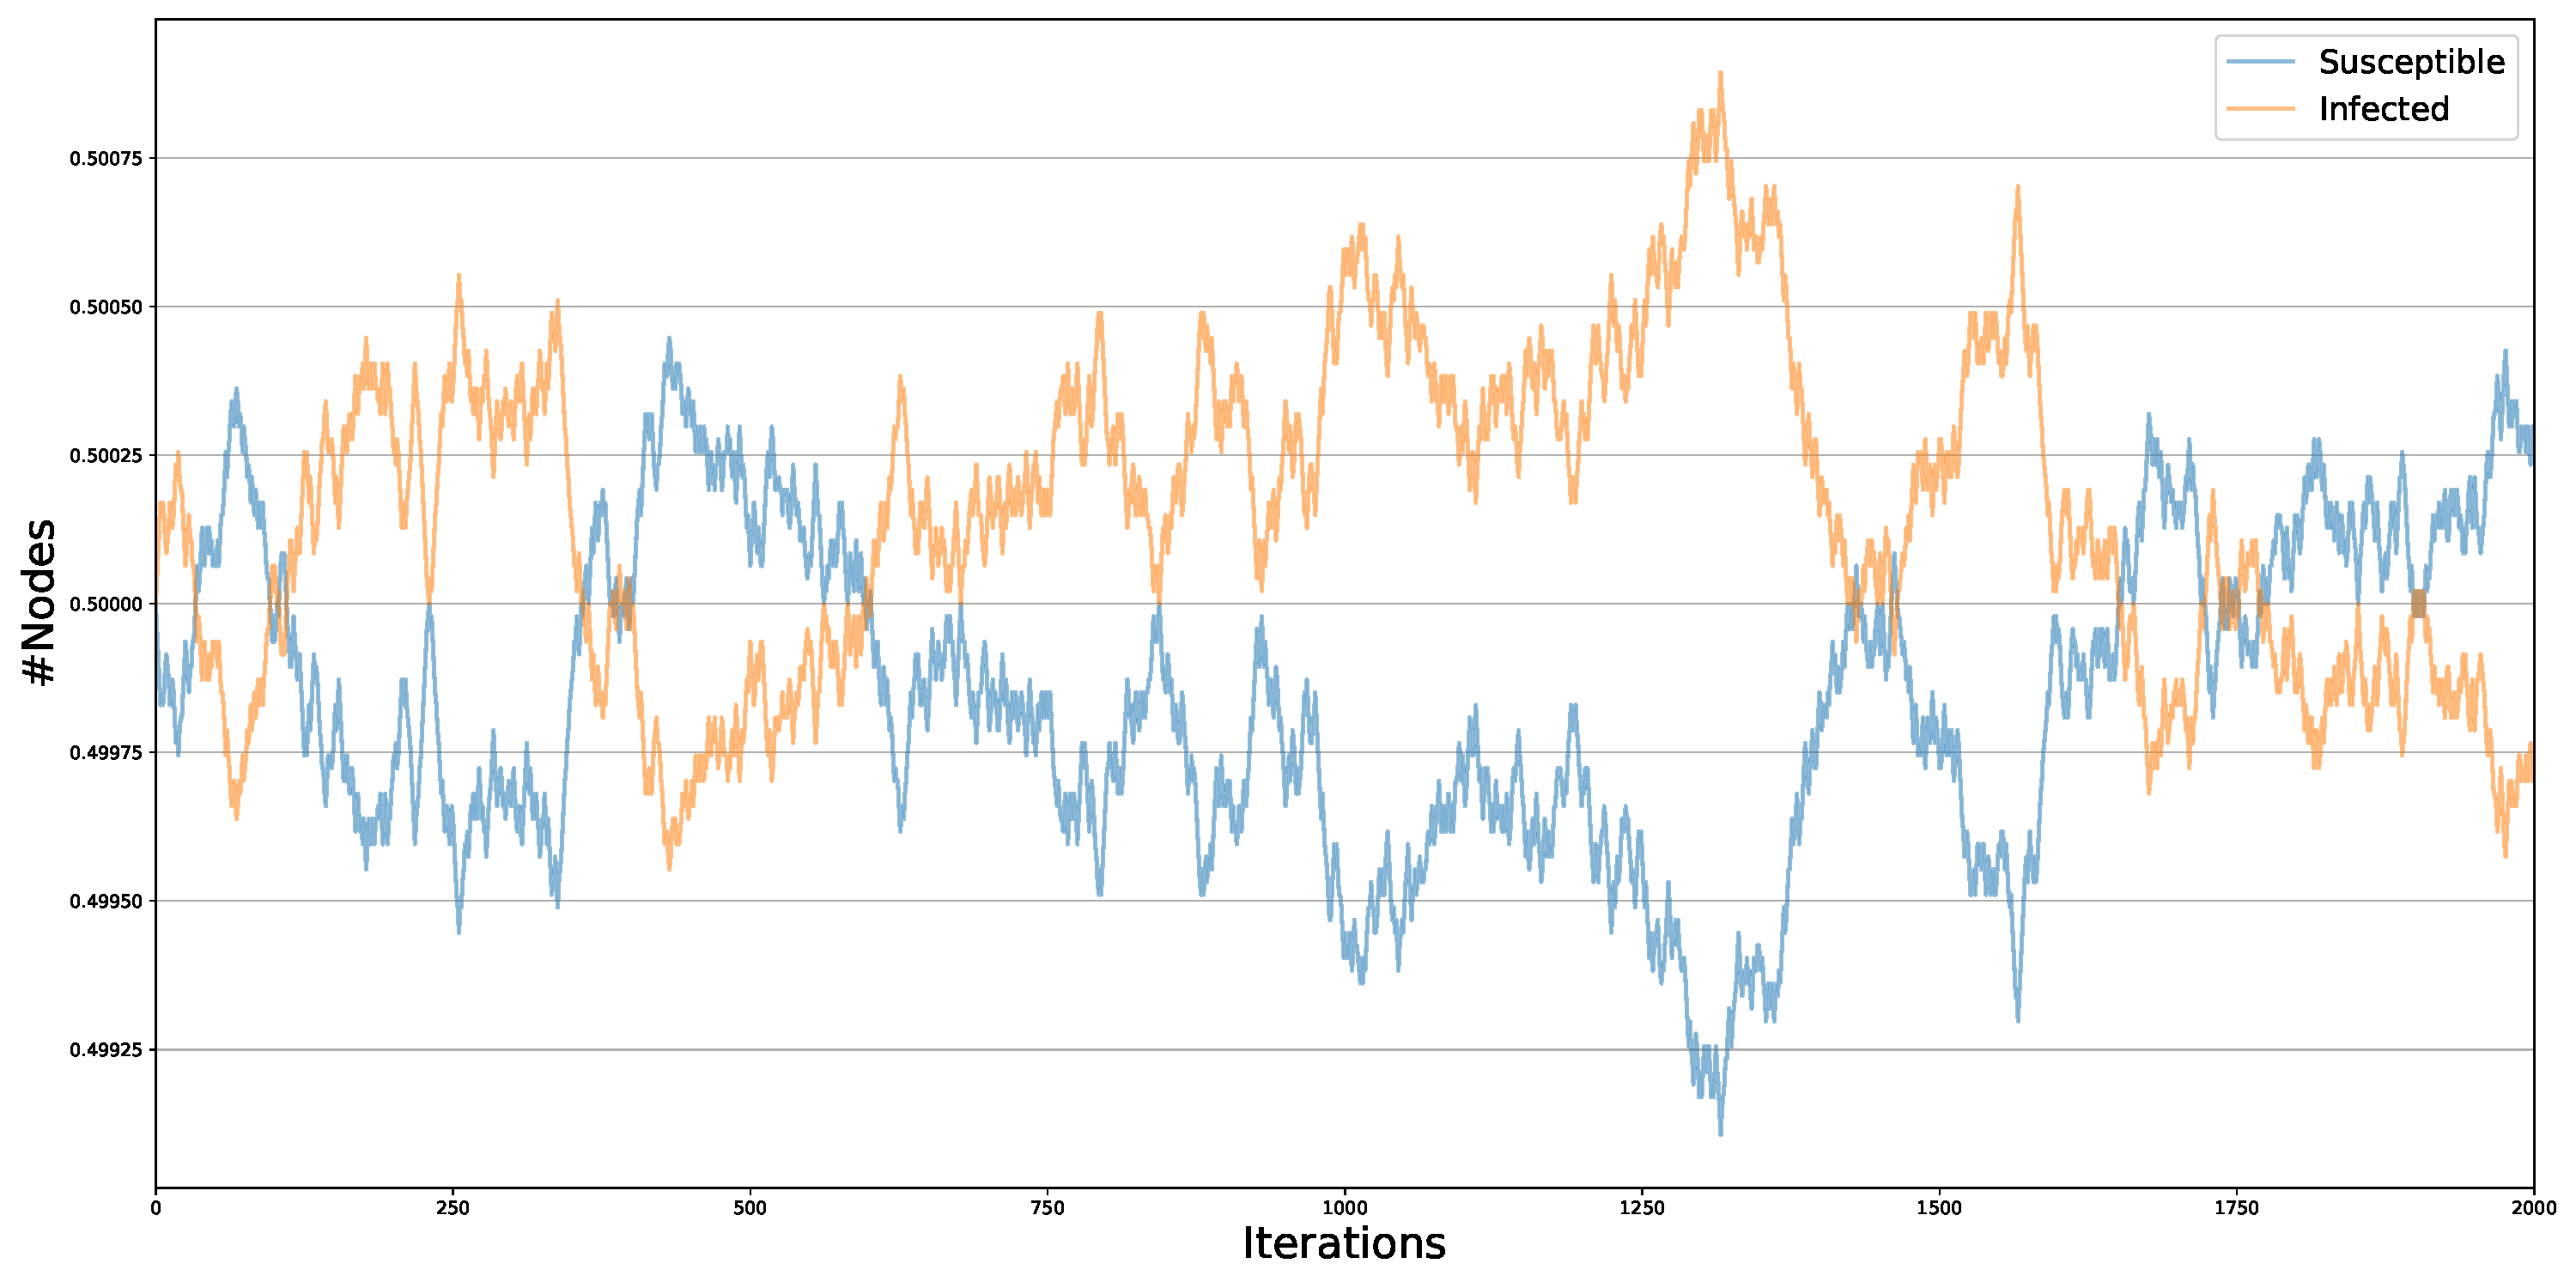
\includegraphics[width=.9\linewidth]{report/img/OD/MajorityRule_0.5.pdf}
   \caption{Real World Network}
   \label{fig:RW_MR} 
\end{subfigure}

\begin{subfigure}[H]{1\columnwidth}
   \centering
   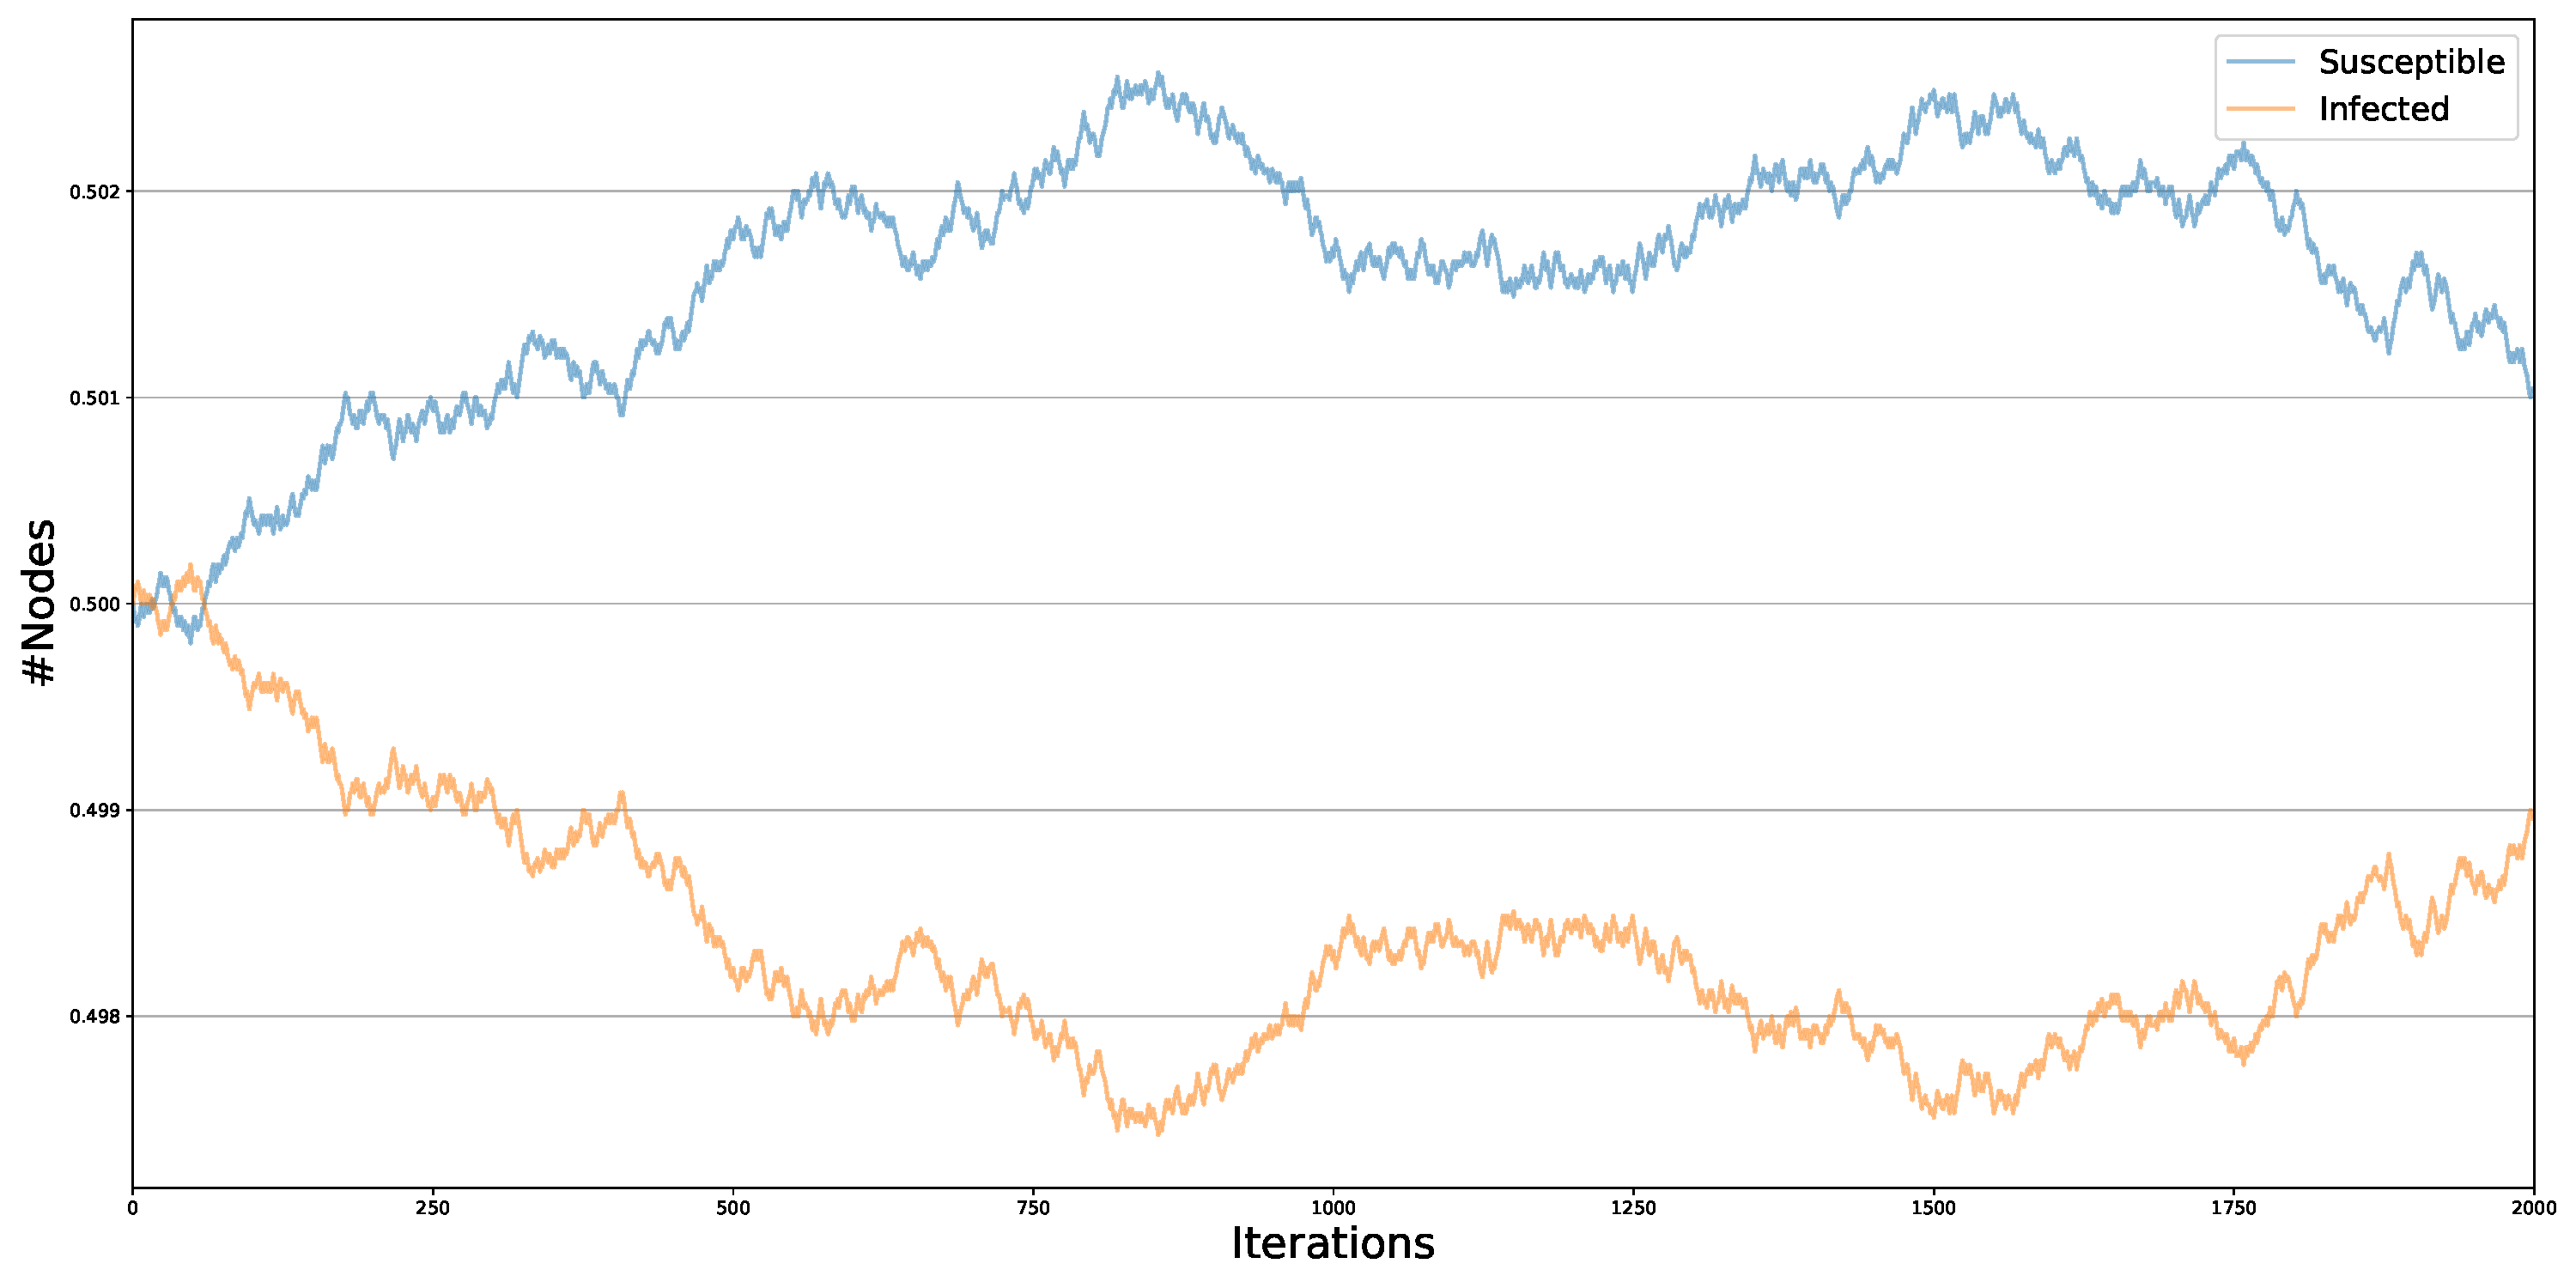
\includegraphics[width=.9\linewidth]{report/img/OD/MajorityRuleBA_0.5.pdf}
   \caption{Barabasi-Albert Network}
   \label{fig:BA_MR}
\end{subfigure}

\caption{Majority Rule Model}
\label{fig:MajorityRule}
\end{figure}

\subsection{Sznajd}
In this context each agent has an opinion ±1. At each timestamp, a pair of neighbouring agents is selected and, if their opinion coincides, all their neighbours take that opinion. 
Given the operation of the model, there is an obvious immediate prevalence of negative opinion in the RW network, as depicted in Figure \ref{fig:RW_Szn}. The situation is different regarding the BA network, in which at the end positive nodes prevail, as shown in Figure \ref{fig:BA_Szn}. To conclude, regarding WS network, the distribution of opinions remains very balanced during the first 1000 iterations, after which an increase in the negative class can be observed in Figure \ref{fig:WS_Szn}.

\begin{figure}[h]
\centering
\begin{subfigure}[h]{1\columnwidth}
    \centering
   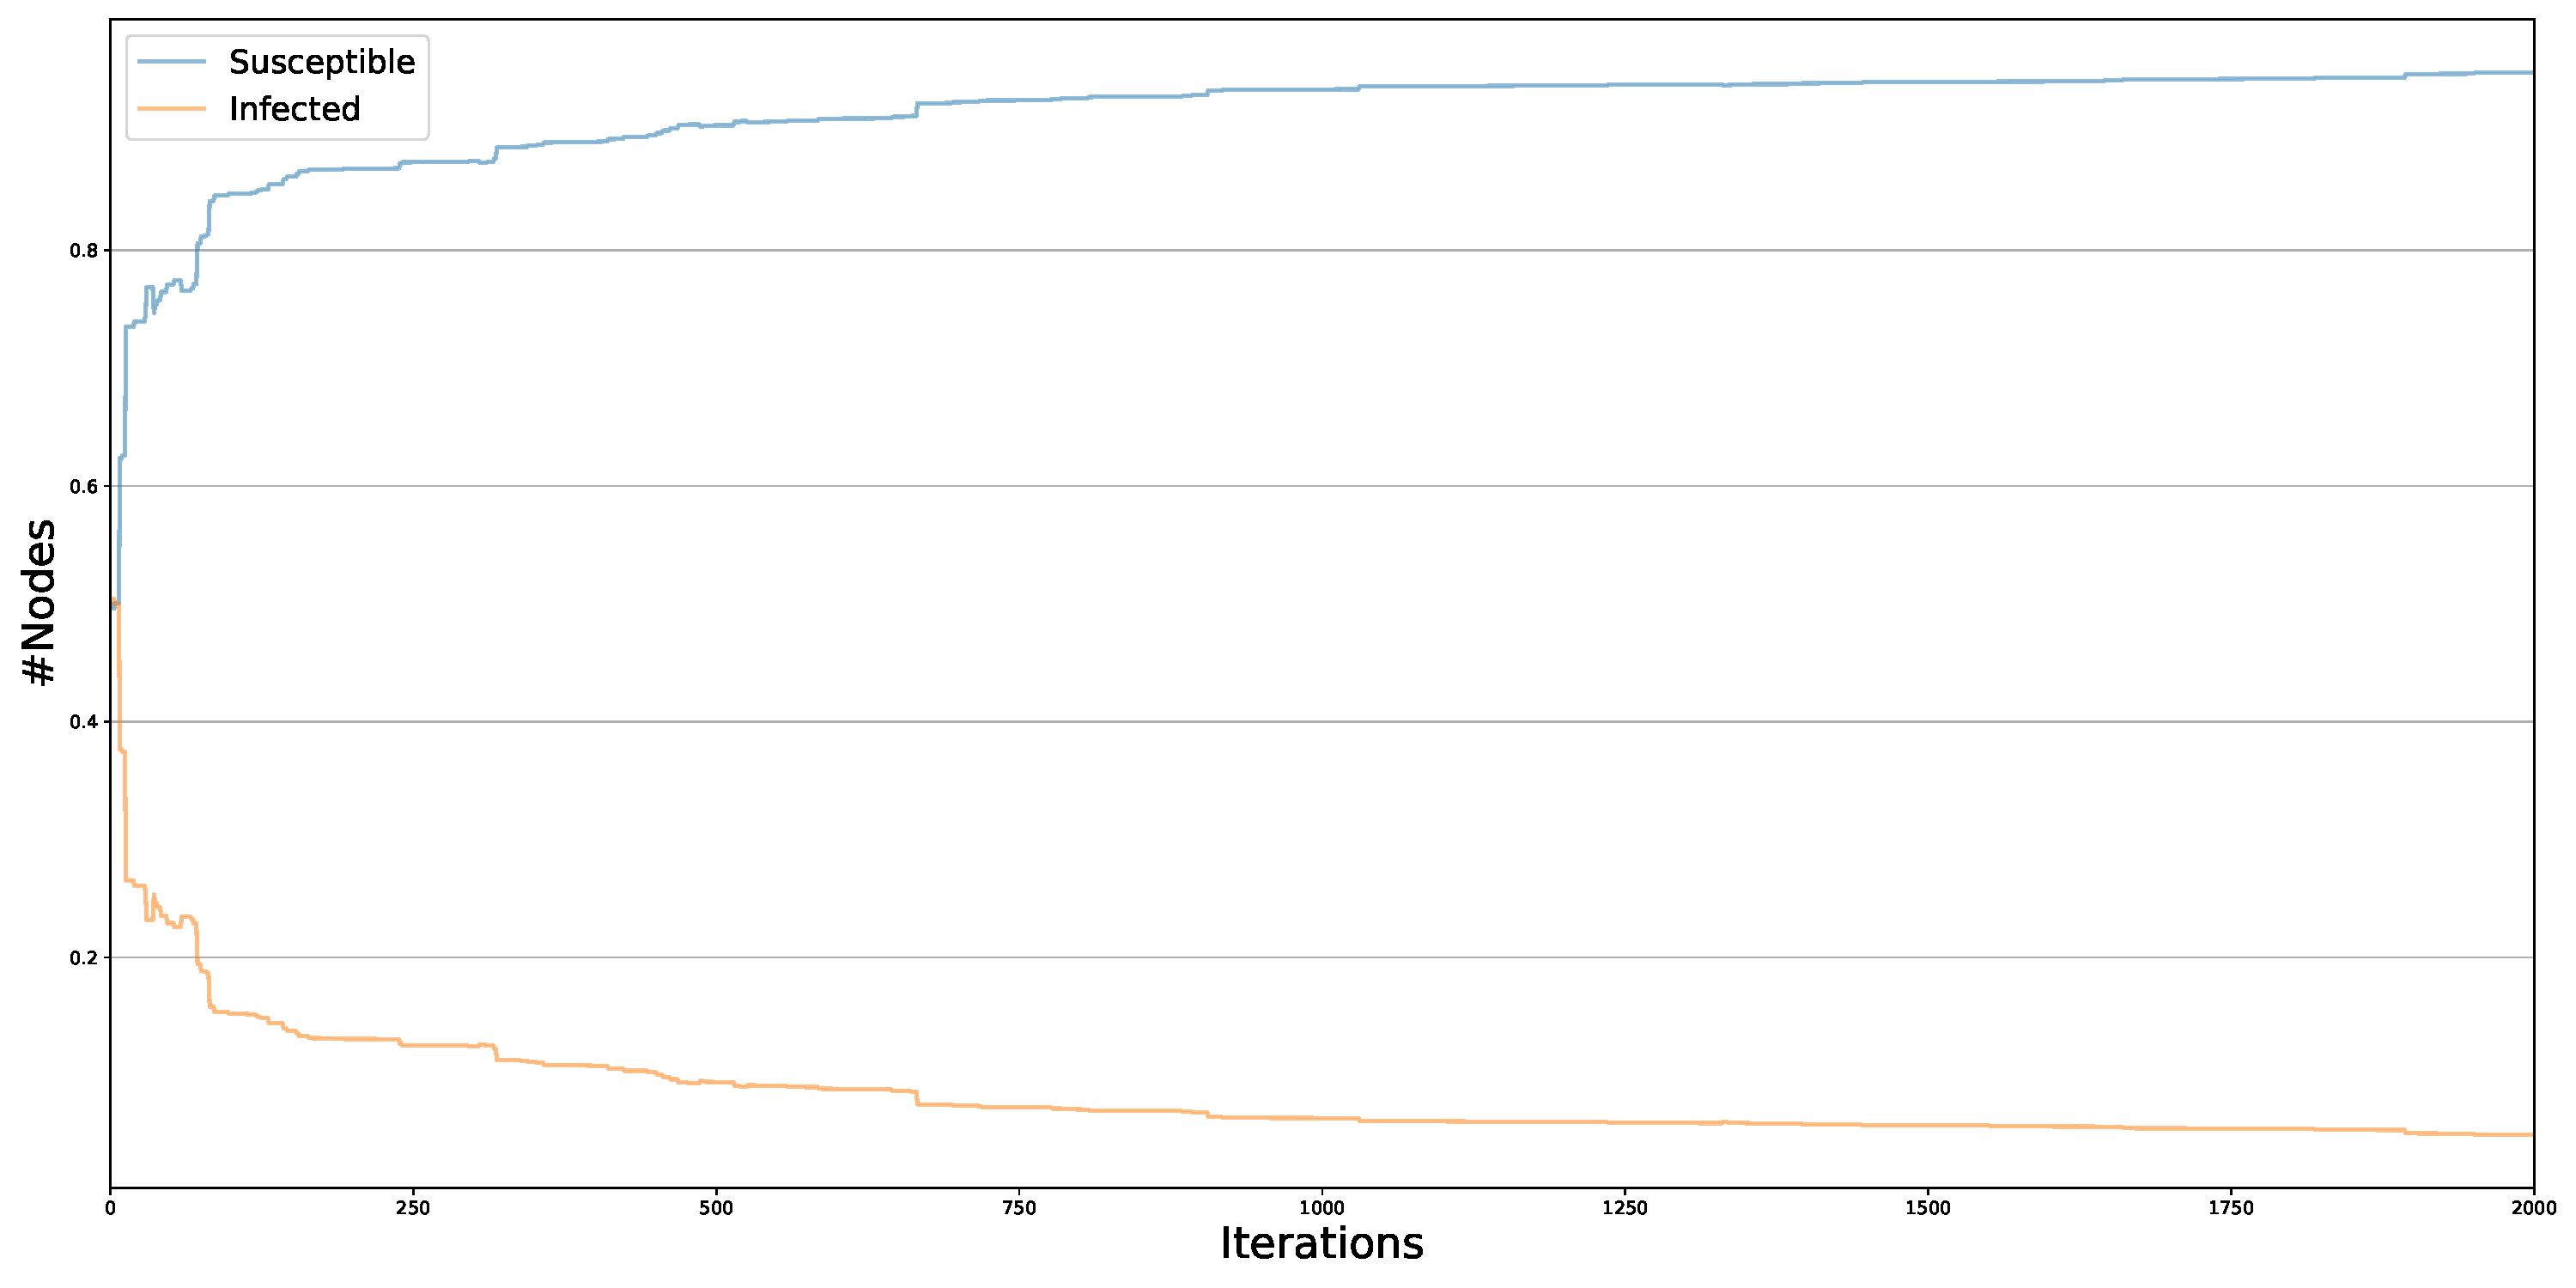
\includegraphics[width=.8\linewidth]{report/img/OD/Sznajd_0.5.pdf}
   \caption{Real World Network}
   \label{fig:RW_Szn} 
\end{subfigure}

\begin{subfigure}[h]{1\columnwidth}
   \centering
   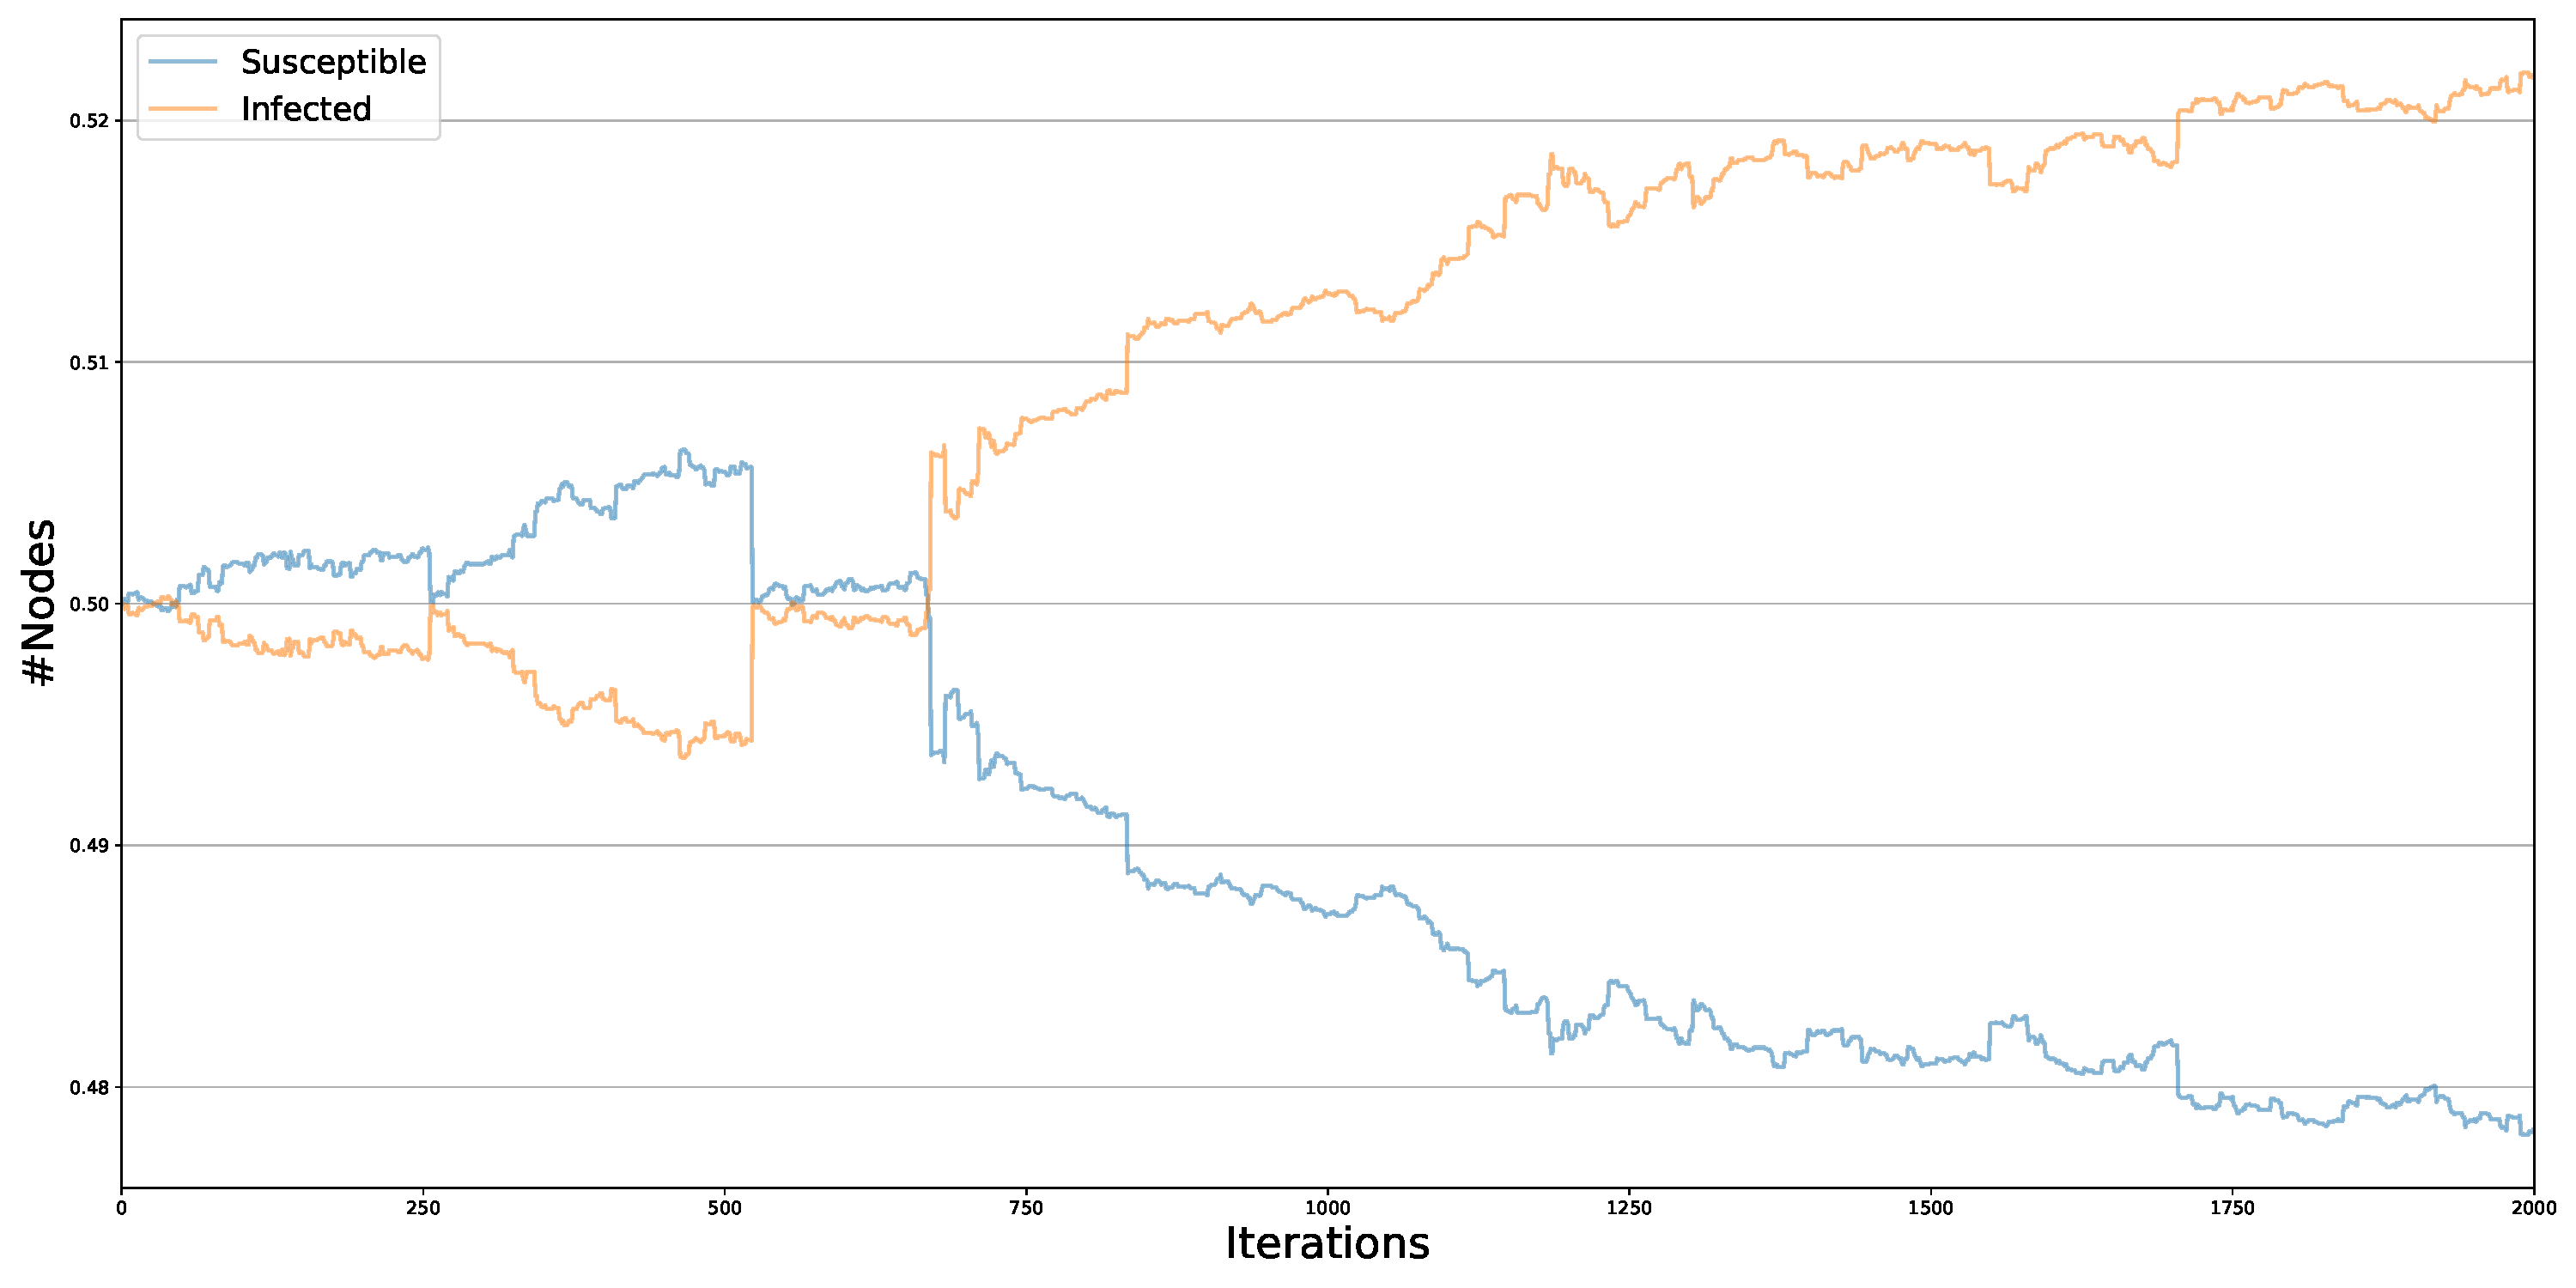
\includegraphics[width=.8\linewidth]{report/img/OD/SznajdBA_0.5.pdf}
   \caption{Barabasi-Albert Network}
   \label{fig:BA_Szn}
\end{subfigure}

\begin{subfigure}[h]{1\columnwidth}
   \centering
   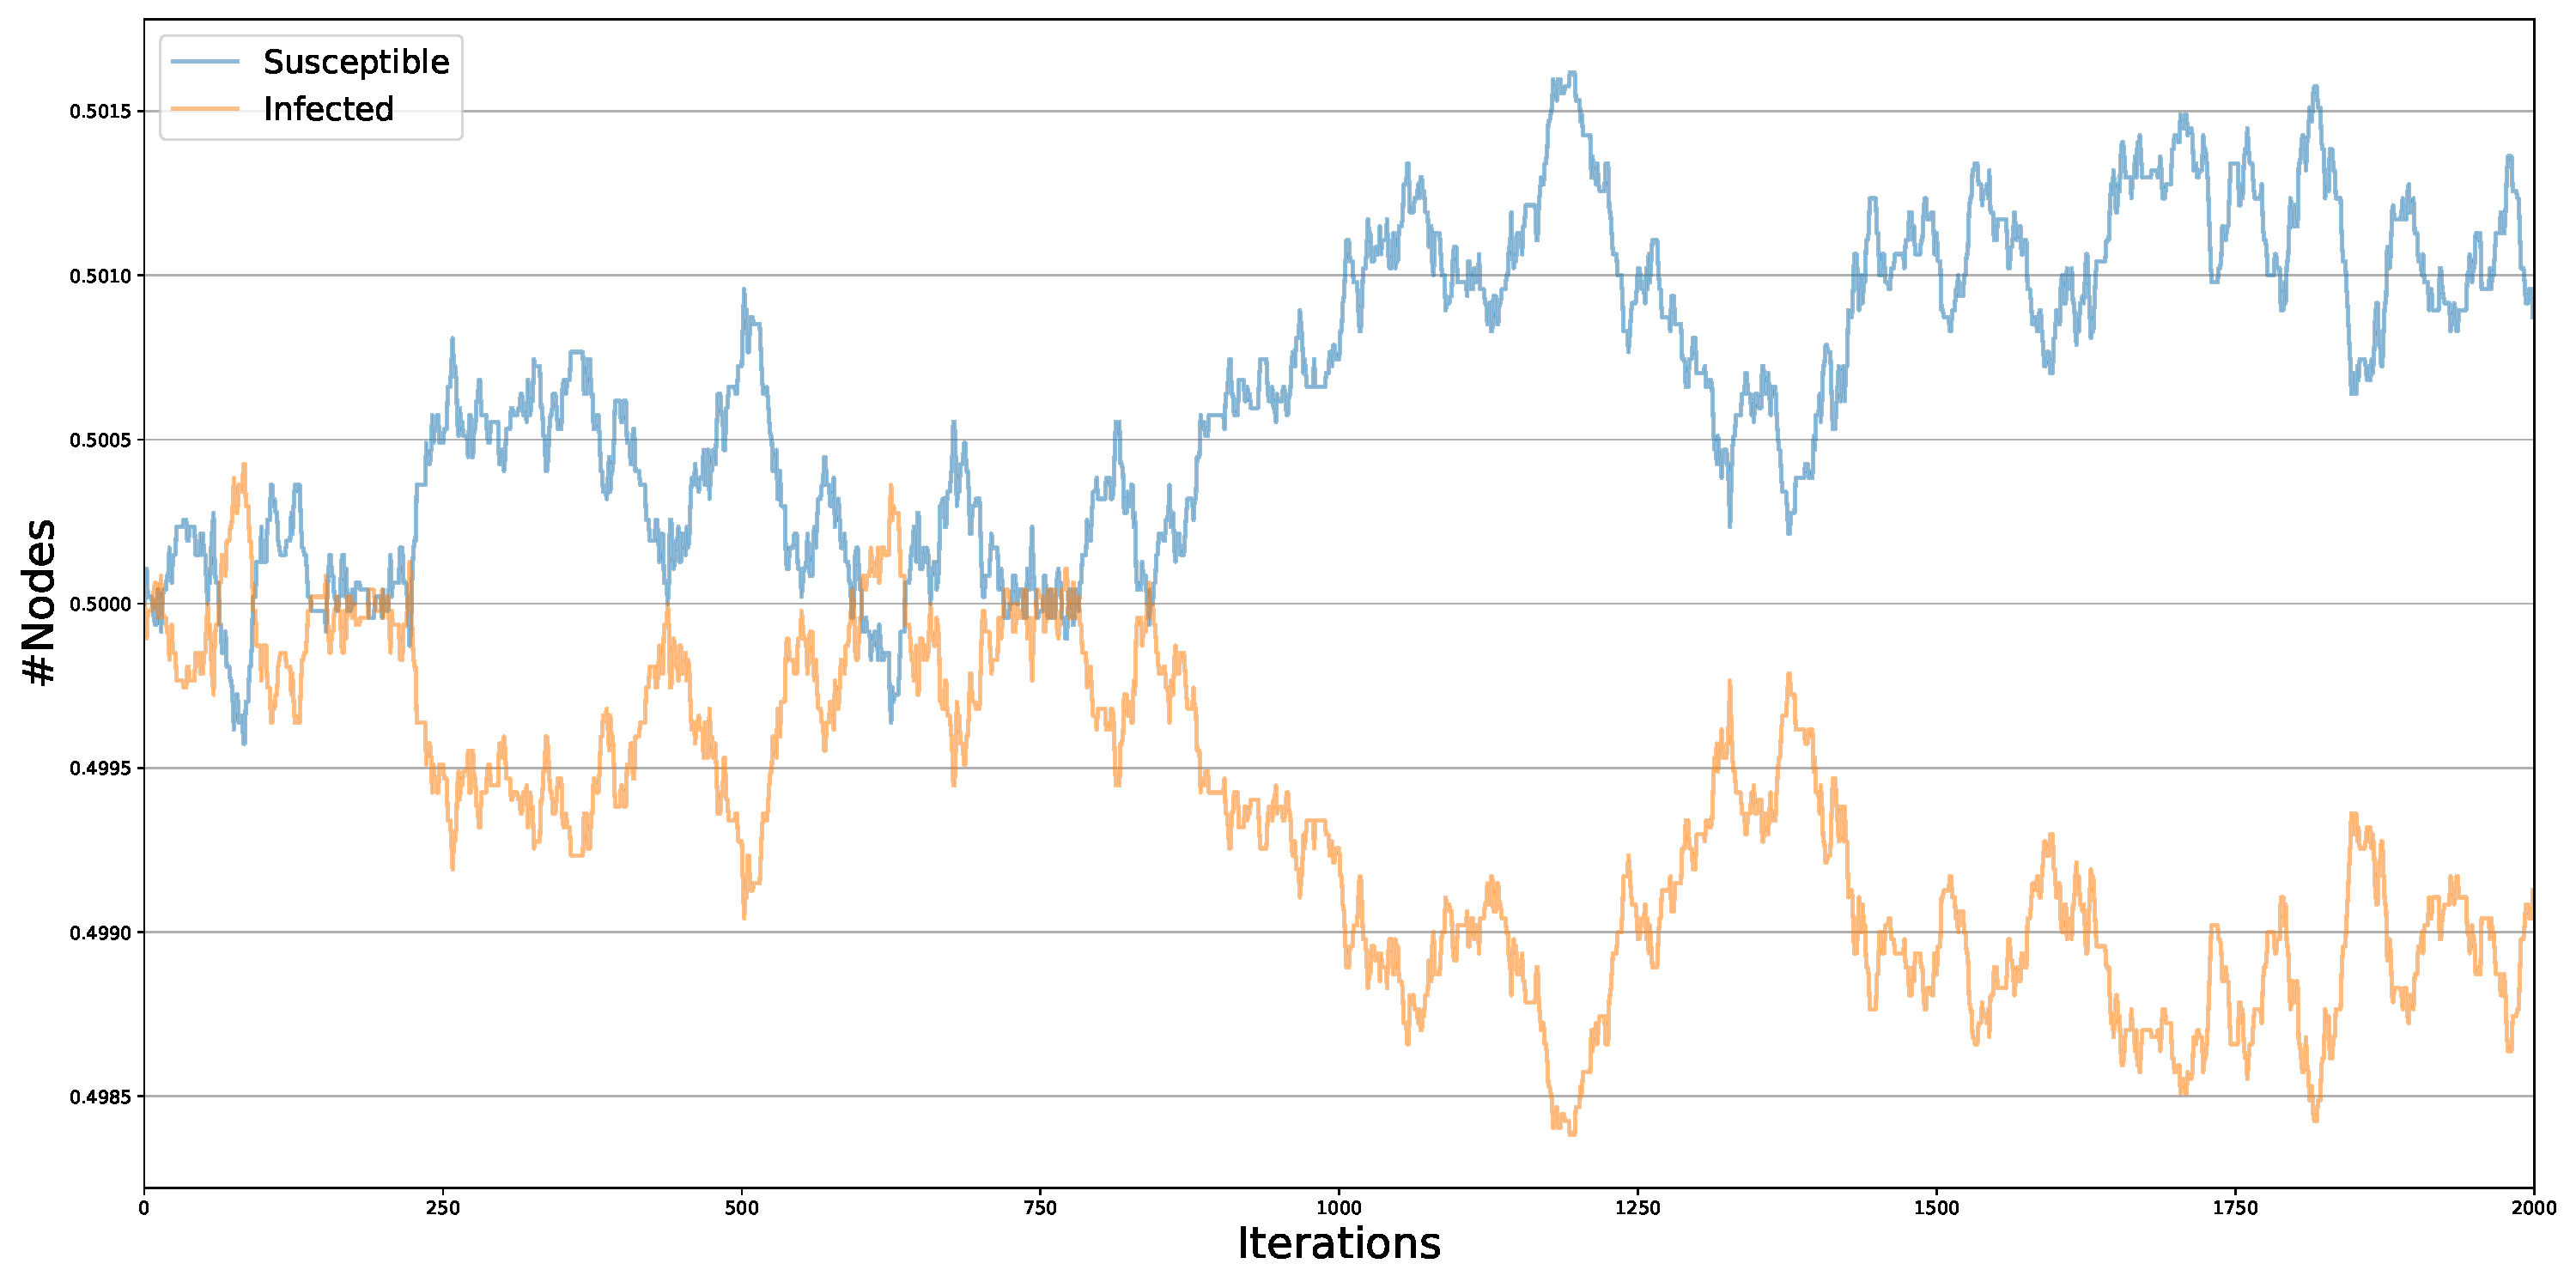
\includegraphics[width=.8\linewidth]{report/img/OD/SznajdWS_0.5.pdf}
   \caption{Watts-Strogatz Network}
   \label{fig:WS_Szn}
\end{subfigure}
\caption{Sznajd Model}
\label{fig:Sznajd}
\end{figure}

\section{Task 3: Open Question}

In this last task, we mostly used the results of the last two ones in order to investigate our main question, i.e. if the Russian invasion of Ukraine had an impact on the opinions of Italians about migrants and refugees.

As a preliminary study, it would be interesting to study if a tweet regarding Ukraine has a more positive sentiment compared to a tweet regarding migrants. In order to do so, the distribution of the user label (calculated in the nodes labeling subsection) was plotted in two cases: if the tweet contained the substring ucr or not. 

\begin{figure}[b]
\begin{subfigure}{.48\columnwidth}
  \centering
  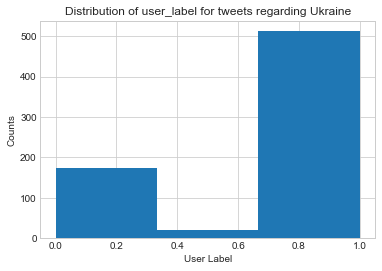
\includegraphics[width=\linewidth]{report/img/ucr3.png}
  \caption{Tweets containing the substring "ucr"}
  \label{fig:ucrtweet}
\end{subfigure}%
\hfill
\begin{subfigure}{.48\columnwidth}
  \centering
  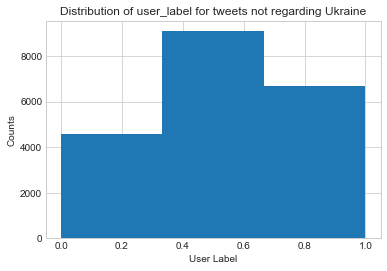
\includegraphics[width=\linewidth]{report/img/rest3.png}
  \caption{Tweets not containing the substring "ucr"}
  \label{fig:resttweet}
\end{subfigure}
\caption{Distribution of the user label in the two cases.}
\label{fig:labeldistribution}
\end{figure}

As one can see, in Figure \ref{fig:ucrtweet} the distribution is massively shifted towards the 1 class, i.e. people having a positive sentiment; while in in Figure \ref{fig:resttweet} the distribution tend to be more uniform compared to the other one. This behaviour can also be seen in the mean of the user label cases: in the first case the mean is 0.72, while in the other 0.51. 
This latter result shows how the tweets regarding Ukraine tend to have a more positive sentiment compared to the others.

In order to look at the change of opinions by the users, it was decided to use the Sankey Plot for a visual representation. This is particularly useful in our situation, since one wants to characterize the amount of shifts in our graph between two or more temporal snapshots. For the creation of this kind of plot, the library \textit{Plotly}\cite{plotly} was used.

The first necessary step to compare the opinions before and after the Russo-Ukrainian conflict is to split the dataset in two frames, using the date of the tweet as a discriminator. In particular, it was chosen to use the date of the Russian invasion of Ukraine (24/2/2022) as split condition. In order to have more statistically relevant results, it was chosen to apply another condition, i.e. it was required that each user wrote at least two tweets in every temporal snapshot. The user label is then recomputed as the mean of each tweet label in each temporal frame. Furthermore, it was decided to bin the user label, creating four categories bins in which the user label is included in:

\begin{itemize}
    \item 0-0.25: negative sentiment about migrants;
    \item 0.25-0.5: slightly negative sentiment about migrants;
    \item 0.5-0.75: slightly positive sentiment about migrants;
    \item 0.75-1: positive sentiment about migrants;
\end{itemize}

The Sankey diagram is finally produced by selecting the users that appear in both temporal snapshot and plotting their shift.

\begin{figure}[h]
    \centering
    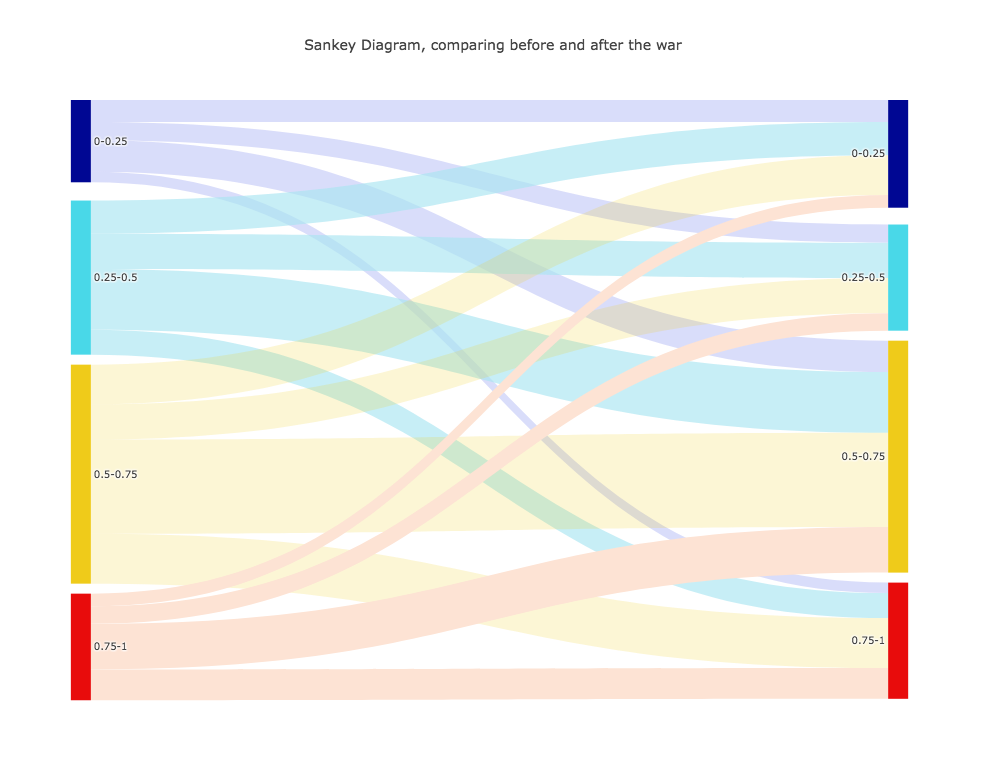
\includegraphics[width=0.9\columnwidth]{report/img/Sankey_before_after_2tweet.png}
    \caption{Sankey Diagram of user label in the two temporal snapshot, before and after the 2022 Russo-Ukrainian conflict}
    \label{fig:sankey_before_after}
\end{figure}

The result shown in Figure \ref{fig:sankey_before_after} highlights the natural behaviour of a user to preferentially stay in the same bin or to move in an adjacent bin, i.e. to have a moderate change of opinion instead of a drastic one.

The other effect one notices is that the bins "0-0.25" and "0.75-1" are bigger in the snapshot after the conflict. This radicalization might be seen as the consequence of the arrival of Ukrainian refugees, or could be an effect due to the proximity of Italian election. Figure \ref{fig:time} shows how a great number of tweets were written after May 2022, with a peak in July 2022, which indicates the start of the electoral campaign for the Italian election of September 2022. In this temporal frame one finds therefore a great number of tweets written by politicians with a well defined opinion on immigration, and as a cascade effect the user might have taken a defined position as well.


In addition to the flux, one could investigate the increase or decrease percentage of every bin count in the two temporal snapshot, in order to have a quantitative measure for the opinion change.

Since the goal is to identify the change of opinion about migrants and refugees, we feared that these numbers might be biased from the presence of the tweets regarding Ukraine, which are positive biased as shown in Figure \ref{fig:ucrtweet}. For this reason it was decided to repeat the analysis on the tweets not containing the substring "ucr". 

It was also considered to repeat this analysis on two temporal snapshots before the war. The idea behind this reasoning is the following: if one compares two temporal snapshot which are not divided by an event so strong to make the people change their mind, one could get a very rough estimation of a natural statistical fluctuation of the counts of the bins. This measure is useful to compare the change in our Before-After study with some statistical fluctuations. 
As temporal frames for the last described comparison were chosen the first two snapshot created in the dynamic community discovery task.

\begin{table}[h]
    \centering
        \caption{Percentual change of bin counts.\\BtA indicates the change of user label from before to after the 2022 Russo-Ukrainian Conflict; BtA/Ukr idem but having removed the tweets containing the substring "ucr"; 1to2 indicates the change between the first and second temporal snapshot created in the dynamic community discovery task.}
     \adjustbox{max width=\columnwidth}{%
    \begin{tabular}{c|c|c|c|c|c|c}
         & 0-0.5 & 0.5-1 &  0-0.25 & 0.25-0.5 & 0.5-0.75 & 0.75-1\\\hline
         BtA & -9\% & +7\% & +31\% & -31\% & +6\% & +9\% \\
         BtA/Ukr & -9\% & +6\% & +33\% & -31\% & +5\% & +9\% \\
         1to2 & -5\% & +4\% & -2\% & -9\% & -0.1\% & +6\% \\
    \end{tabular}
    }
    \label{tab:changebins}
\end{table}


The results of this analysis is presented in Table \ref{tab:changebins}. For a better visualization, a bar chart of these data is reported in in Figure \ref{fig:percbar}.
Besides the change of each bin, it could be interesting to look at the sum of the classes in the bins "0-0.25", "0.25-0.5" and "0.5-0.75", "0.75-1", which are now bins indicating the negative and positive sentiment. As one can see, the rows BtA and BtA/Ukr are similar and there is no significantly change, although it was noticed the small effect of the slightly smaller increase of the positive 0.5-1 class, with the consequent increase of the negative sentiment class, as predicted. This effect is small and therefore negligible. 
Comparing the changes in 1to2, these are significantly smaller than the one in the row BtA. This may be a hint that the Russo-Ukrainian conflict (and also the Italian election) could have had an effect on the Italians' opinion about migrants.

\begin{figure}[h]
    \centering
    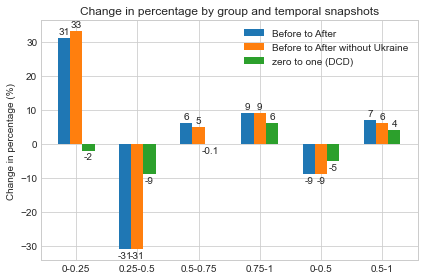
\includegraphics[width=0.88\columnwidth]{report/img/change_percentage.png}
    \caption{Percentage change of bin counts per temporal snapshots succesion}
    \label{fig:percbar}
\end{figure}


The overview results of the graph can be visualized with the tool \textit{Gephi}. One can visualize the distribution of the user label, which is represented by a colorization coherent with the Sankey plot of Figure \ref{fig:sankey_before_after}. In particular, in Figure \ref{fig:graphbefore} there is a dominance of cold colors indicating a majority of negative sentiment, while in Figure \ref{fig:graphafter} the graph is dominated by warm colors, indicating a positive sentiment. There is furthermore another effect identifiable by the graph visualization, which is the color distribution inside of hubs. These aggregation of nodes represent the conversation in which take part a great amount of users. As one can notice, the hubs are mainly constituted by blue or red users, which represent the most extreme categories (respectively 0-0.25 and 0.75-1). This effect indicates that in the most discussed topics the most polarized users take the word, leaving less space to the people with a more undefined opinion.

\begin{figure}[h]
  \centering
  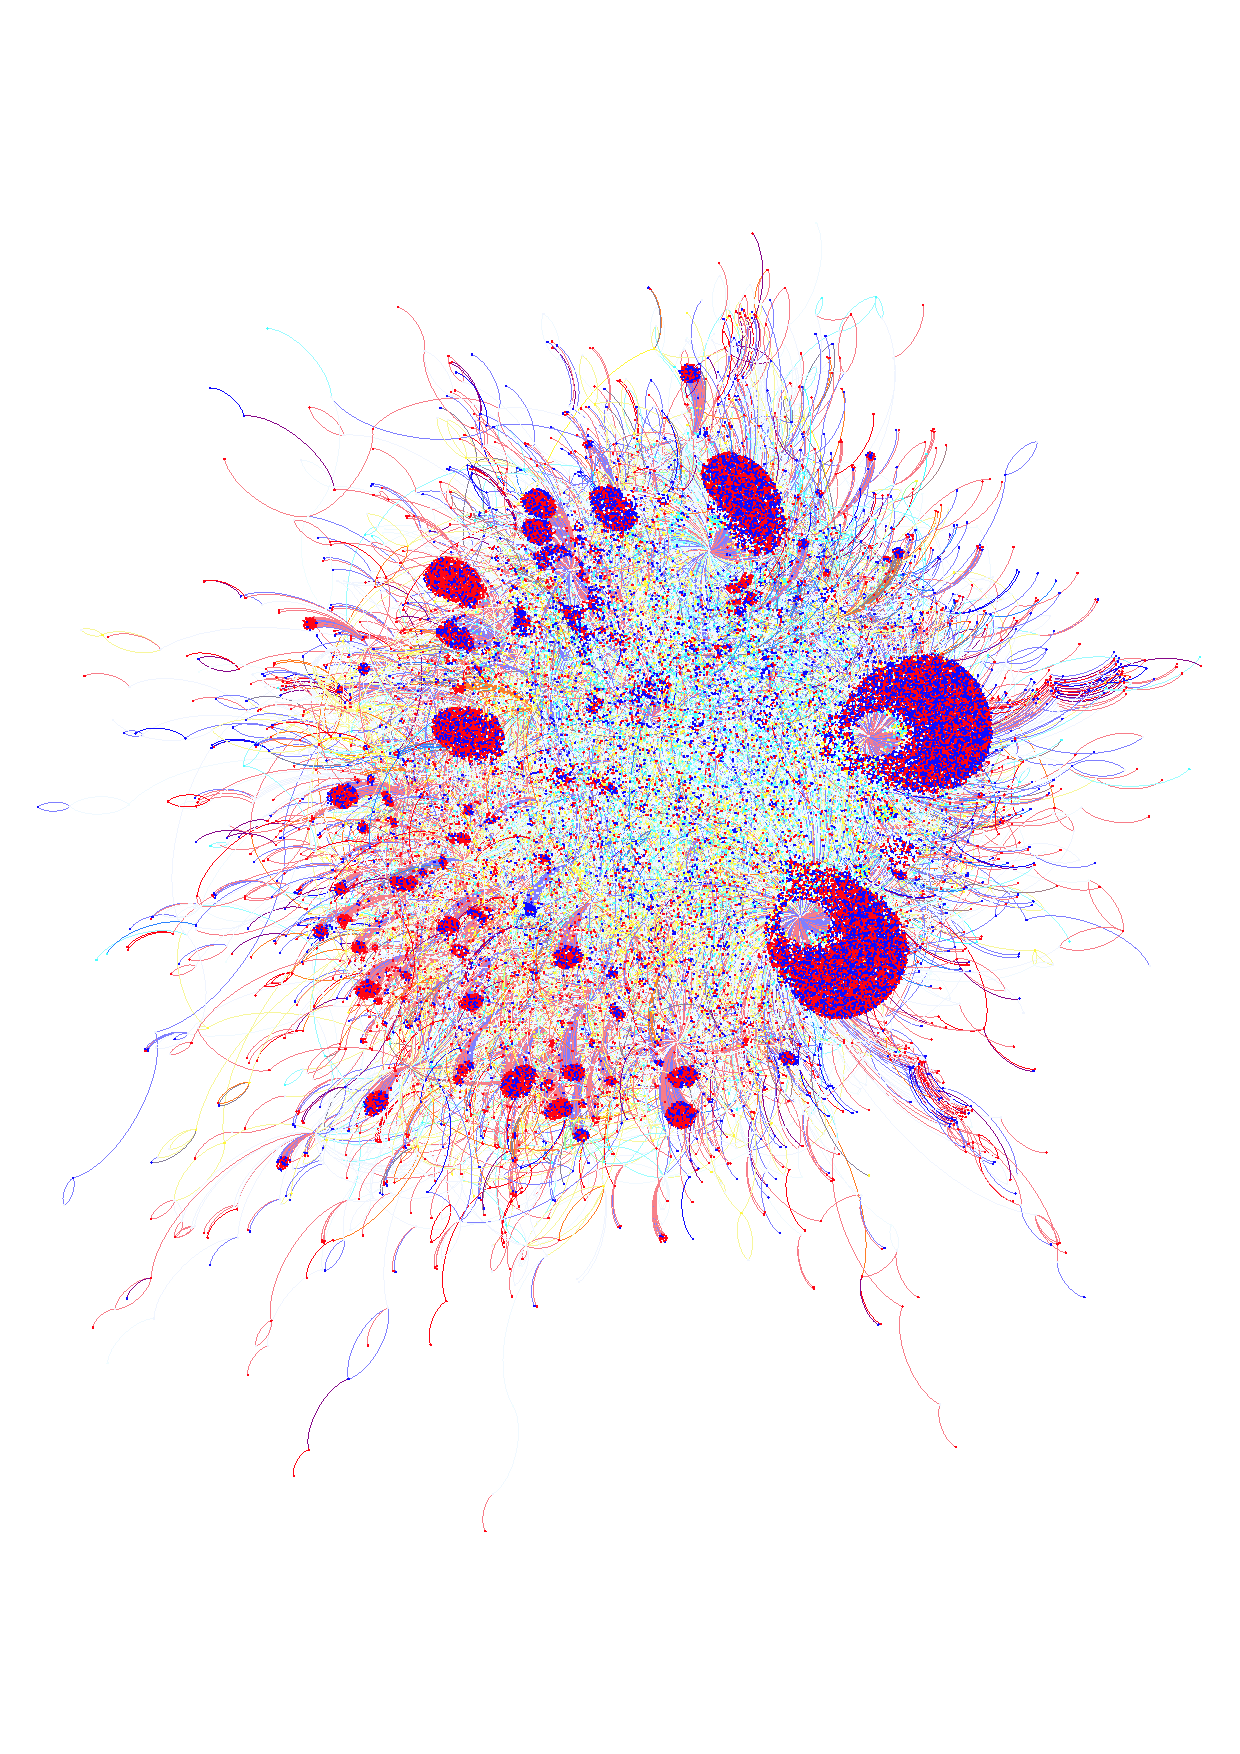
\includegraphics[width=0.88\columnwidth]{report/img/graph_before_sparso.pdf}
  \caption{Graph before the Russo-Ukrainian conflict}
  \label{fig:graphbefore}
\end{figure}%

\begin{figure}[h]
  \centering
  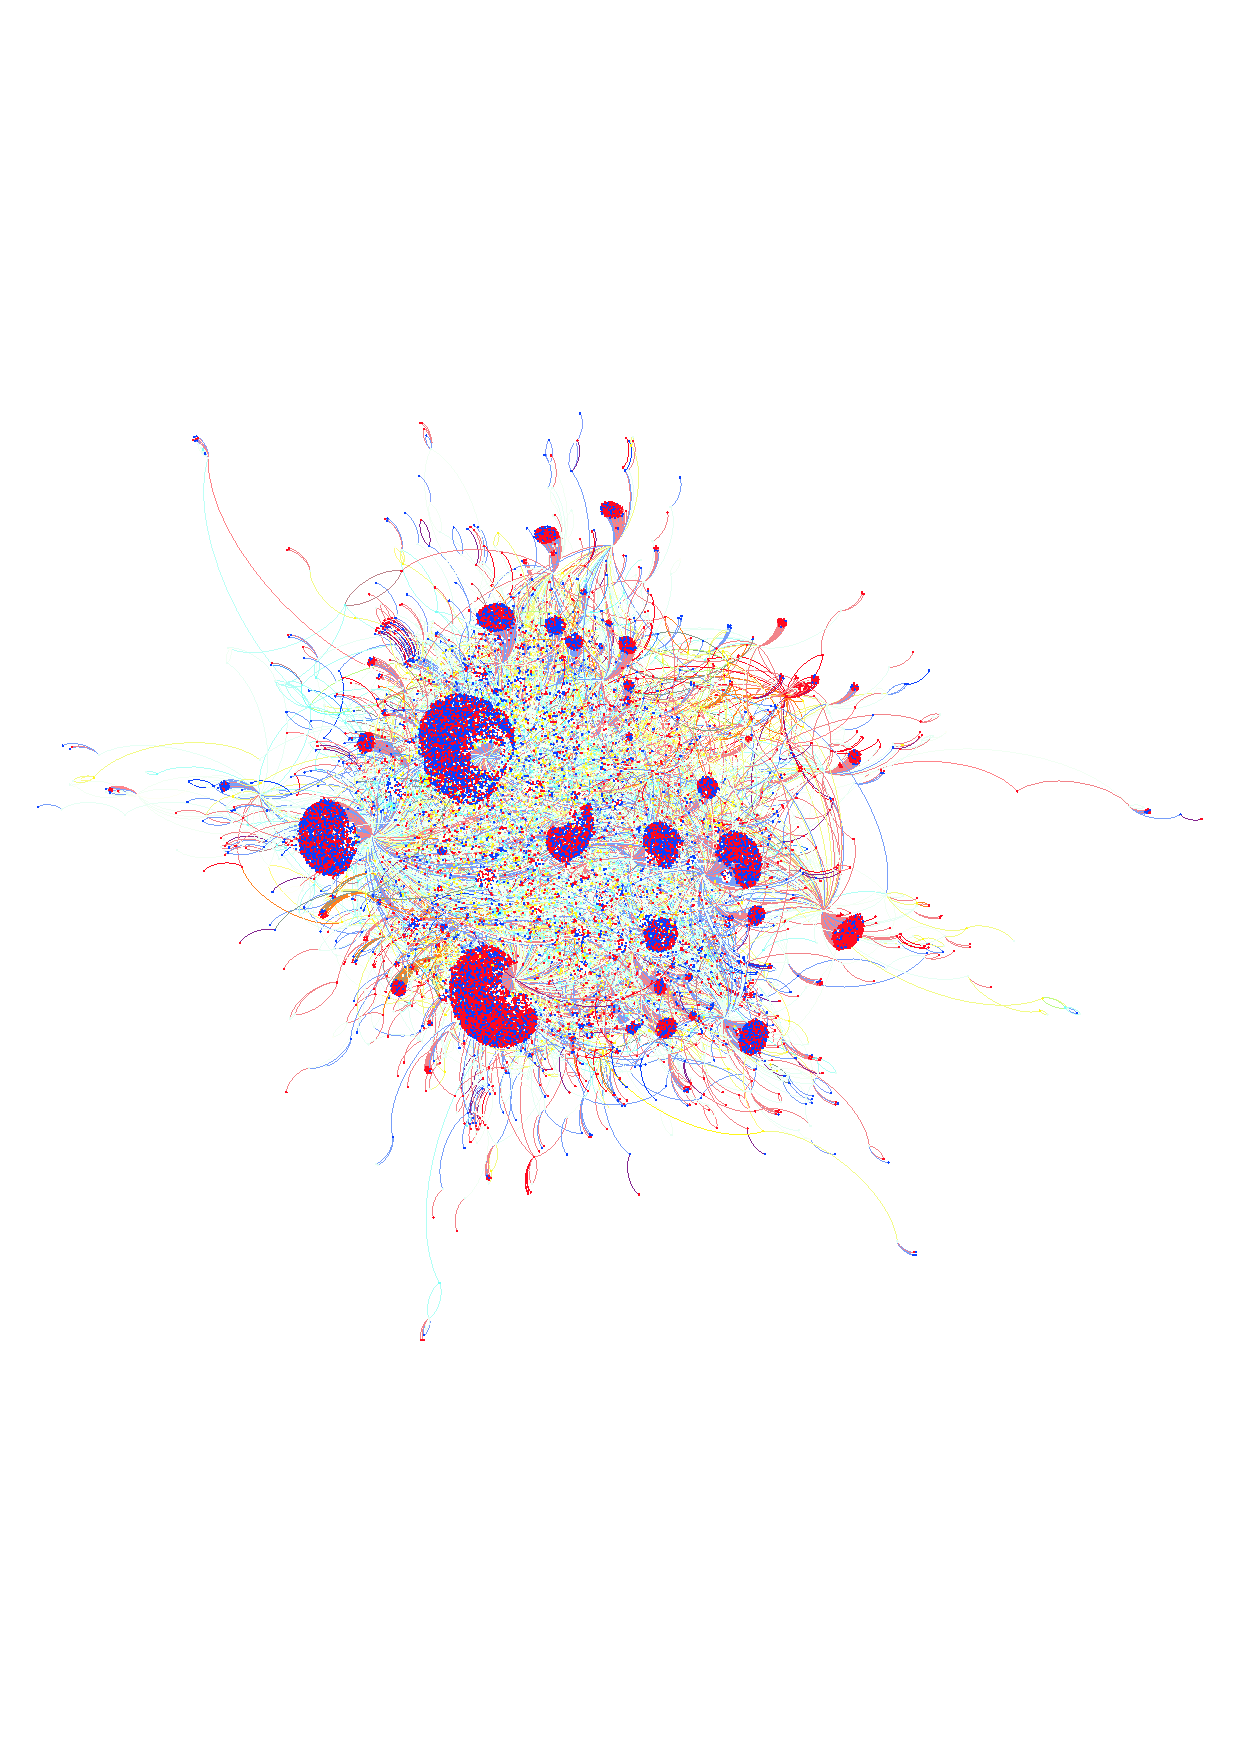
\includegraphics[width=0.98\columnwidth]{report/img/graph_after_sparso.pdf}
  \caption{Graph after the Russo-Ukrainian conflict}
  \label{fig:graphafter}
%\caption{Graph visualization of the temporal snapshots. The color of the nodes follows the same grading of the Sankey diagram in Figure \ref{fig:sankey_before_after}.}
%\label{fig:graph}
\end{figure}



\section{Discussion}
In this project an analysis about Italians' opinion regarding refugees and migrants in general has been carried out. To do so, through the python library \textit{snscraper}, data about tweets and users has been collected starting from September 2020 until September 2022. This specific temporal window has been chosen because the main goal of the analysis was to capture a change in opinions following the Russian-Ukrainian conflict. The data has been  manipulated by tools and algorithms offered by \textit{Network Science} and \textit{Data Mining} knowledge in general. As a preliminary step, in order to obtain an indicator about the opinion of the user, it has been created a new attribute called \textit{User\_Label} based on the mean-sentiment of tweets wrote by each User. Then, the topology of the obtained network has been explored in order to catch some useful information about which nodes were hubs or generally more influential in the discussion comparing different centrality measures. 

As a first task, in Section 4, \textit{Community Discovery} has been carried out, both in a static and dynamic way. In particular, the latter allows to reach the most relevant considerations, due to the temporal dimension. In fact, time was a key variable for whole analysis. The contribution of this task was crucial during the conduct of the open question, allowing a more complete interpretation of the results.

Before moving to the last task, different \textit{Opinion Dynamic} models have been run on the network (both in the real world and in synthetic ones) with the aim of observing the way opinions change over time, from positive to negative and vice-versa. Comparing the \textit{voter model} on the real-world network with the Barabasi-Albert one, the greatest similarity in terms of spreading was found.

All the results obtained from the previous tasks were merged, in order to try to give an answer to the main paper's topic. Even though from the analysis of tweets containing the substring "ucr" emerges a prevalence of pro-refugees opinion, it is not exactly the same by taking the whole network. Moreover, the first two columns in Table \ref{tab:changebins} highlights a mild shift from a negative opinion to a positive one, when classifying an opinion between 0 and 0.5 as 0 and an opinion between 0.5 and 1 as 1. However, looking at the more detailed opinions in four bins, it can be noticed that the stronger effect regards the increasing of the 0-0.25 bin (+31\%). These effects are also visible in the Sankey diagram depicted in Figure \ref{fig:sankey_before_after}, which also shows that the major contribution to this bin is coming from the 0.5-0.75 one, i.e. a non-negligible amount of people who had a slightly positive sentiment before the war found themselves having a strong negative feeling about migrants after the war.
In conclusion, since the conflict is a fairly recent event, the data collected is not sufficient to derive statistically relevant and reliable results. We suggest, therefore, that the analysis be repeated when more data are available to work with.

% The next two lines define the bibliography style to be used, and the bibliography file.
%\newpage
\bibliographystyle{ACM-Reference-Format}
\bibliography{biblio}

\end{document}

